% 学習結果説明（手順5：シフト構造の本実装。構造 B・A・C × H の扱い (1)(2)(4)。用語集と図の見方）
% results フォルダで「lualatex 学習結果説明_手順5.tex」を2回実行すると PDF を作り直せる（TeX Live の LuaLaTeX を使用）。
% 図は results/step5/ の PNG を相対パスで読み込む。
\documentclass[paper=a4paper,fontsize=10.5pt,line_length=44zw,number_of_lines=38]{jlreq}
\usepackage[haranoaji]{luatexja-preset}
\usepackage{amsmath}
\usepackage{graphicx}
\usepackage{booktabs}
\usepackage{tabularx}
\usepackage{enumitem}
\usepackage{float}
\usepackage{xcolor}
\usepackage[hidelinks,bookmarksnumbered]{hyperref}
\graphicspath{{step5/}}

\newcommand{\file}[1]{\texttt{\detokenize{#1}}}
\newcommand{\gd}{\dot{\gamma}}
\newcommand{\Tff}{T_{\mathrm{ff}}}
\newcommand{\Tset}{T_{\mathrm{set}}}
\newcommand{\Eh}{E_{h}}
\newcommand{\Ev}{E_{v}}
\newcommand{\PI}{P3\_1}
\newcommand{\PII}{P3\_2}
\newenvironment{termlist}{\begin{itemize}[label=・,leftmargin=1\zw,labelwidth=1\zw,labelsep=0pt,itemsep=0.4ex,topsep=0.6ex,parsep=0pt]}{\end{itemize}}
\newcommand{\term}[1]{\item \textbf{#1}：}
\newenvironment{points}{\begin{itemize}[label=$\triangleright$,leftmargin=1.5\zw,itemsep=0.3ex,topsep=0.5ex,parsep=0pt]}{\end{itemize}}
\newcommand{\pt}[1]{\item \textbf{#1}：}
\renewcommand{\arraystretch}{1.25}

\title{樹脂粘度モデル開発　手順5の学習結果の説明\\[0.6ex]{\large シフト構造の本実装（構造 B・A・C $\times$ 厚み $H$ の扱い (1)(2)(4)）：用語集とグラフの見方（機械学習・統計を初めて学ぶ人向け）}}
\author{}
\date{2026年10月14日}

\begin{document}
\maketitle
{\small\tableofcontents}

% =====================================================================
\section{この文書について}

この文書は、\file{results/step5/} にある手順5の結果（図と表）を、機械学習や統計を初めて学ぶ人でも読めるように説明したものです。手順5 は、「温度が変わると流動曲線がずれる」という構造（温度シフト構造）を、実際のデータで本格的に試す手順です。

\begin{points}
\pt{対象の結果}\file{results/step5/}：図 32 枚、CSV 10 個。図は、すべて \file{results/step5/highres/} にも 600 dpi で保存されます（ほかに、せん断速度 ― 粘度のグラフ 56 枚）。
\pt{読み方}2章で何を比べたかをつかみ、分からない言葉は3章の用語集で調べてください。4章で図の見方、5章で表の見方、6章で結論と、これからの選択肢を説明します。\textbf{結論だけを知りたいときは、6章から読んでください}。
\pt{元のノート}\file{01_機械学習コードフォルダ} の \file{手順5_シフト構造の本実装.ipynb} です。実行は約 2.6 時間です（設定で短くできます）。
\pt{記号表}記号・モデル名・列名の一覧は、\file{学習結果説明_記号表.pdf} にあります。
\pt{作り直し方}\file{results} フォルダで \texttt{lualatex 学習結果説明\_手順5.tex} を2回実行すると、この PDF を作り直せます。
\pt{ノートの判定}ノートの各節の最後に、\file{>> 判定：OK}（想定どおり）か \file{>> 判定：★要確認}（想定と違う、または注意が要る点）が出ます。今回は、OK が 107 個、★ が 46 個でした。★ はエラーではなく、「結果を読むときに気をつける点」の目印です。6章に、★ の意味を書きました。
\end{points}

% =====================================================================
\section{何を比べたか（概要）}

\subsection{温度シフト構造とは}
同じ樹脂でも、温度を変えると、せん断速度 $\gd$ と粘度 $\eta$ の関係（流動曲線）の位置が変わります。温度を変えたときの曲線のずれを、「ずらし方の決まった式」で表したものが\textbf{温度シフト構造}です。ずらす量は、アレニウス型の式
\[ \ln a(T;E) = \frac{E}{R}\Bigl(\frac{1}{T}-\frac{1}{T_{\mathrm{ref}}}\Bigr) \]
（$T$ は温度 [K]、$T_{\mathrm{ref}}$ は基準温度 210 ℃ = 483.15 K、$R$ は気体定数）で決まり、$E$ が大きいほど大きくずれます。この $E$ は、文献の活性化エネルギー（PP の流動で 40 kJ/mol 前後）とは別物で、このデータの「見かけの粘度」の温度依存性を表す、データから決める係数です。

\begin{table}[H]
\caption{比べた構造（$f$ はガウス過程で表す「基準の流動曲線」。$u=\ln\gd+\ln a(\Tset;\Eh)$、$w=\ln\mathrm{Fo}$ は冷却の度合い）}\label{tab:struct}
\begin{tabularx}{\linewidth}{@{}l>{\raggedright\arraybackslash}p{13\zw}X@{}}
\toprule
記号 & 式 & 何を表すか \\
\midrule
B（本命） & $\ln\eta=\ln a(\Tset;\Ev)+f(u,\,w)$ & 温度で、曲線が横（$\gd$ の向き、$\Eh$）にも縦（粘度の向き、$\Ev$）にもずれる \\
A（対案） & $\ln\eta=\ln a(\Tset;\Ev)+f(\ln\gd,\,w)$ & 縦だけずれる（B の $\Eh=0$）。同じ $\gd$ で、低温ほど一定の倍率だけ粘い \\
C（基準） & $\ln\eta=f(\ln\gd,\,\ln H,\,\Tset)$ & 構造を入れず、$\Tset$ を、ほかの入力と同じように並べた通常の GPR（手順3b・3d の R3） \\
\bottomrule
\end{tabularx}
\end{table}
構造 B・A が C と同じくらいの精度で、特に学習の範囲の外（外挿）で C を上回れば、「温度シフト構造は、データで支持された」と考えます。構造があると、温度の効果が少ないパラメータ（$\Eh$・$\Ev$）で表せて、解釈もしやすくなります。

\subsection{厚み $H$ の扱い (1)(2)(4)}
手順3e で、厚み $H$ はリークではないが、見かけの粘度は厚みで大きく違う（0.5 mm は 2.0 mm の約 2 倍以上）と分かりました。そこで、$H$ の扱いを次の 5 通りにして、構造ごとに比べました（ユーザーの決定、10 月 14 日）。

\begin{table}[H]
\caption{$H$ の扱い（$m$：材料の部分、$c$：厚み・冷却の補正。B・A の $u$ は横シフト後の $\gd$、C は $\ln\gd$ と $\Tset$）}\label{tab:hv}
\begin{tabularx}{\linewidth}{@{}l>{\raggedright\arraybackslash}p{9\zw}X@{}}
\toprule
扱い & 形 & 意味 \\
\midrule
(1) & $f(u,w)$ & $H$（フーリエ数 Fo）を、入力に残す。基本形 \\
(2) & $m(u)+c(w)$ & Cross-WLF のように、材料の部分 $m$ と、厚み・冷却の補正 $c$ に、足し算で分ける \\
(4) & $f(u,p)$ & $H$ を使わず、圧力 \PII\ を入れる（$p=\ln\PII$） \\
(1+4) & $f(u,w,p)$ & $H$ と \PII\ の両方 \\
(2+4) & $m(u,p)+c(w)$ & (2) に \PII\ を足す \\
\bottomrule
\end{tabularx}
\end{table}
構造 3 通り $\times$ 扱い 5 通り = 15 モデルです。名前は「構造\_扱い」（例：B\_1、A\_2、C\_4）。C\_1 は R3、C\_4 は W2 と同じモデルです。

\subsection{(2) と (4) の注意}
\begin{points}
\pt{(2) の足し算}$m$ と $c$ は、「定数だけ入れ替えられる」ので、図では $c$ の平均を 0 にそろえて見せます。$m$ は $\gd$ と温度の関数（Cross-WLF にあたる）、$c$ は $\ln\mathrm{Fo}$ だけの関数です。
\pt{(4) の P3\_2}\PII\ は、流れの結果として測る値で、成形条件から予測するときには事前に分かりません。さらに、\PII\ は厚みでほぼ決まる量（$H^{-1.5}$ に比例）で、$H$ の代わりの目印として働きます。そこで、(4) を含むモデルは 2 通りで評価しました。
\begin{itemize}[itemsep=0.2ex,topsep=0.3ex]
\item \textbf{実測の \PII}：検証の条件の、実測の条件平均を使う。「\PII\ が分かっている場合」の上限。
\item \textbf{予測した \PII}：事前に分からないとして、$(\ln\gd,\ln H,\Tset)$ から GPR で \PII\ を予測し、その予測のばらつきも含めて ln η を予測する（20 回引いて、平均と分散にまとめる）。
\end{itemize}
2 つの差が、「(4) の良さは、\PII\ が分かっているおかげか」を表します。\PII\ を予測するのにも $H$ が要る点に注意してください。
\end{points}

\subsection{データと評価}
手順3d の 2 つの学習データを使います（どちらも外れ値なしで、問題データ一覧の「除外」を除く）。
\begin{itemize}[itemsep=0.2ex,topsep=0.3ex]
\item \textbf{5data 版}：5data（93 条件）で学習し、3data（36 条件）で検証する。S\_V（射出速度の両端への外挿。低速側・高速側）と S\_T（190・230 ℃ で学習して 210 ℃ を検証）。
\item \textbf{Alldata 版}：全条件で学習。CV（条件単位の 10 分割の交差検証）と S\_T（テストは 5data 版と同じ行）。
\end{itemize}
$E$ は、学習データごとに、その学習データだけで推定します（CV の分割ごとにも推定。検証の情報は使いません）。入力の $\gd$ は条件平均（成形条件から見た予測）です。

% =====================================================================
\section{用語集}
\begin{termlist}
\term{プロファイル尤度}$E$ を格子（決まった間隔の値）で振り、各 $E$ について、GPR を学習して「対数周辺尤度」を求めたもの。$E$ と尤度の関係の図（尤度曲線）が山になっていれば、その山の頂点が、データに最も合う $E$。
\term{対数周辺尤度（LML）}データが、そのモデルで、どれだけ「ありそう」か。大きいほどデータに合う。差が 2〜3 以上なら、はっきりした違い。
\term{1.92 以内の範囲}LML が最大から 1.92 以内の $E$ の範囲。おおよその 95\% 信頼区間（尤度比検定）。範囲が狭いほど、$E$ がデータで決まっている。
\term{$\Delta$LML（\file{dLML_vs_E0}）}$E=0$（温度の効果なし）との LML の差。大きいほど、温度の効果がデータで支持される。
\term{$\Eh$・$\Ev$・$E_v-E_h$}B の 2 つの $E$。尤度の山が斜めの帯になると、2 つは別々には決まらず、差 $E_v-E_h$ だけが決まる。
\term{フーリエ数（Fo）}冷却の度合い。$\ln\mathrm{Fo}=-(\ln\gd+3\ln H)$ ＋ 定数で、$H$ と $\gd$ から計算できる（$H$ と同じ情報）。
\term{足し算のカーネル}$m$ と $c$ を足し算で表すために、2 つのカーネル（$m$ の部分、$c$ の部分）を足したもの。それぞれが、決まった入力の列だけを見る。
\term{マスターカーブ}温度シフトでずらしたあとの、すべての温度のデータを重ねた 1 本の曲線。3 つの温度の点がよく重なれば、その構造でシフトできている。
\term{被覆率}95\% 予測区間に、実測が入った割合。0.95 が理想。
\term{RMSE}予測と実測の差の平均的な大きさ（$\ln\eta$ で。0.05 なら粘度で約 5\%）。
\term{NLPD}負の対数予測密度。当たり具合と区間の適切さをまとめた指標。小さいほどよい。
\term{純粋誤差・ノイズ}同じ条件のショット間のばらつき（$\ln\eta$ の標準偏差、約 0.04）。成形条件だけを入力にしたモデルは、これより小さい誤差にはなれない。
\term{外挿・内挿}学習の範囲の外・内側での予測。
\term{実測の \PII、予測した \PII}2.3 節。
\term{CV（交差検証）}データを 10 に分け、1 つずつ検証に回して、全部の予測をまとめて評価する。同じ条件のショットは同じ側に入れる。
\term{局所解}最適化が、本当の最大でなく、途中の小さな山で止まること。尤度曲線が、でこぼこになる原因。今回は、前の格子点の解を次の初期値にして減らした。
\end{termlist}

% =====================================================================
\section{図の見方}

\subsection{図1：A のプロファイル尤度（Alldata 版）}
\begin{figure}[H]
\centering
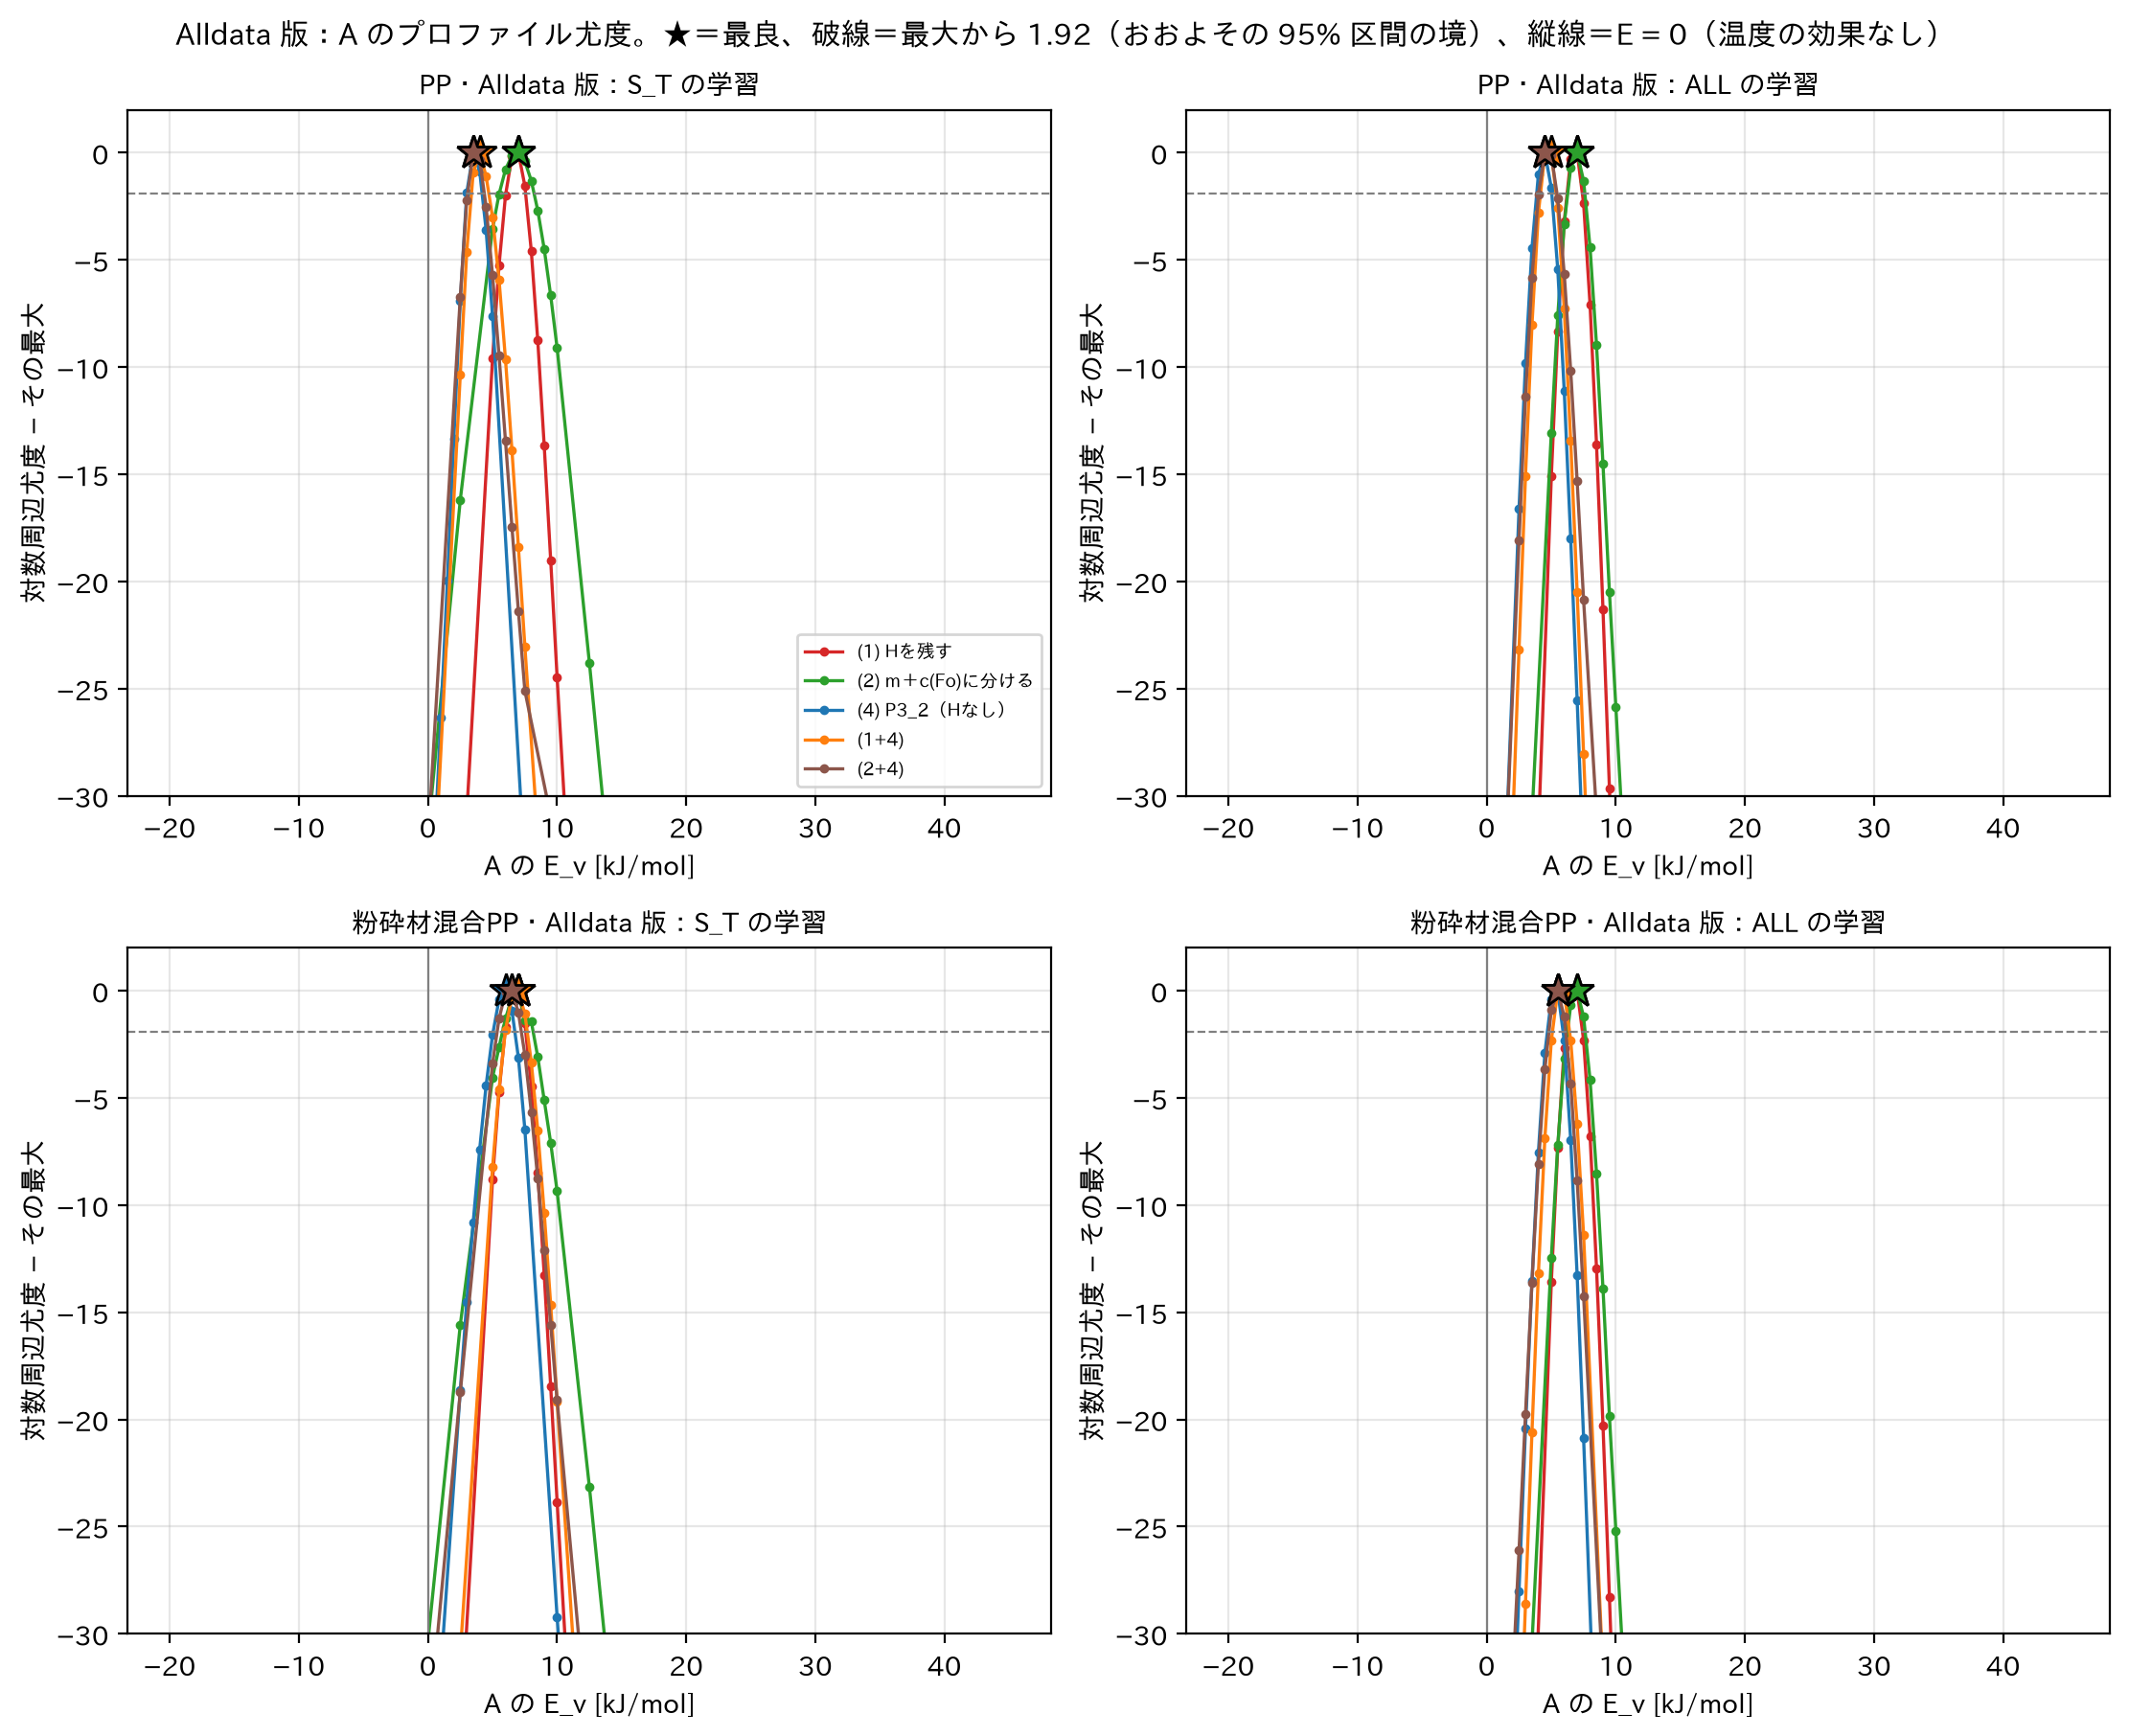
\includegraphics[width=0.97\linewidth]{fig1_profile_A_Alldata.png}
\caption{A の $\Ev$ と、対数周辺尤度の最大との差（上：PP、下：粉砕材混合 PP。左：S\_T の学習、右：ALL の学習。色は $H$ の扱い）}
\end{figure}
\begin{points}
\pt{何を示す図か}A（縦だけシフト）の $\Ev$ を横軸に振り、各 $\Ev$ で学習して求めた対数周辺尤度を、その最大との差で描いた図（尤度曲線）です。山の頂点（★）が、データに最も合う $\Ev$ です。（ファイル：\file{fig1_profile_A_Alldata.png}。\file{highres/} に 600 dpi 版もあります）
\pt{軸と記号}横軸は $\Ev$ [kJ/mol]、縦軸は「対数周辺尤度 $-$ その曲線の最大」（0 が頂点）。灰色の破線が $-1.92$（おおよその 95\% 区間の境）、縦線が $E=0$（温度の効果なし）。色は $H$ の扱い。
\pt{見るポイント}山がはっきりしていて、頂点が $E=0$ から離れているか。山が鋭いほど、$E$ がデータで決まっている。$H$ の扱いで頂点がずれるか。
\pt{今回の結果}どの扱いでも山は鋭く、頂点は $E=0$ から離れています（温度の効果は、データで支持されます）。$\Ev$ は、$H$ を残す (1)(2) で 7.0（PP）・7.0（粉砕材混合 PP）kJ/mol、\PII\ を入れる (4)(1+4)(2+4) で 4.5〜5.0 kJ/mol と、少し小さくなります。190/230 ℃ の粘度比は $\exp(0.0207\,\Ev)$ で、約 1.15 倍です。
\end{points}

\subsection{図2：B の 2 次元プロファイル（PP・Alldata 版）}
\begin{figure}[H]
\centering
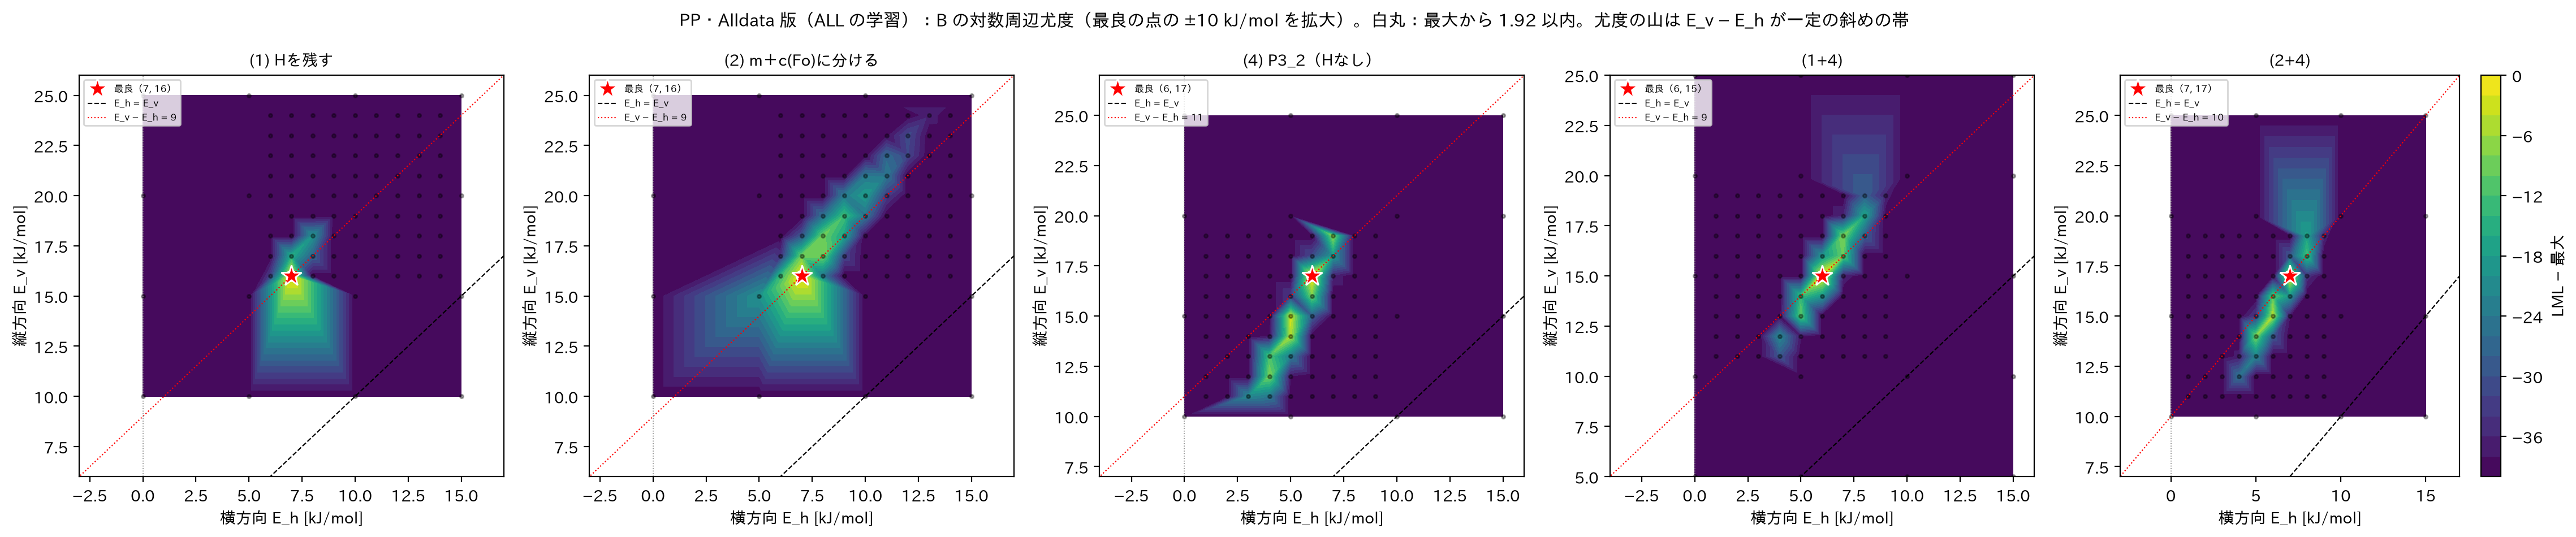
\includegraphics[width=1.0\linewidth]{fig2_profile_B_Alldata_PP.png}
\caption{B の $(\Eh,\Ev)$ の対数周辺尤度（最良の点の $\pm10$ kJ/mol を拡大。列が $H$ の扱い）}
\end{figure}
\begin{points}
\pt{何を示す図か}B（横と縦を別々にシフト）では、$\Eh$（横）と $\Ev$（縦）の 2 つを決めます。2 つの値の組ごとに学習して求めた対数周辺尤度を、色で描いた図です。（ファイル：\file{fig2_profile_B_Alldata_PP.png}。\file{highres/} に 600 dpi 版もあります）
\pt{軸と記号}横軸が $\Eh$、縦軸が $\Ev$（kJ/mol）。黄〜緑が尤度の高い所（最大に近い）、紫は最大より 40 以上低い所。赤い星が最良の点、白丸が最大から 1.92 以内の点、黒い小点が計算した格子の点。黒い破線が $\Eh=\Ev$（当初の構造 H）、赤い点線が、最良の点を通る $\Ev-\Eh=$ 一定の線。
\pt{見るポイント}尤度の山が、星のまわりに、細い斜めの帯（赤い点線に沿った帯）になっていれば、「$\Eh$ と $\Ev$ は、差だけがよく決まる」ことを表します。帯の幅（白丸の範囲）が狭いほど、$\Eh$・$\Ev$ がデータで決まっています。
\pt{今回の結果}山は、赤い点線に沿った細い斜めの帯で、星のまわりの狭い範囲に絞られました。$H$ を残す (1) では、白丸の範囲は星の 1 点（$\Eh$ は $\pm$1 kJ/mol 程度）で、$\Eh=7$・$\Ev=16$ kJ/mol、差 $\Ev-\Eh=9$ です。(2)(4)(1+4)(2+4) では、帯が少し長く、斜めに伸びますが、差は 8〜11 kJ/mol の範囲に収まっています（表\ref{tab:E}）。手順5a では、「$\Eh$ と $\Ev$ は別々には決めきれない」と書きましたが、今回は、前の格子点の解を初期値にして局所解を減らし、細かい格子で調べた結果、$\Eh$ も数 kJ/mol の幅に絞れました（ただし、細かい格子の範囲は最良の点の $\pm$4 kJ/mol までなので、帯の長さは、この範囲までしか分かりません）。
\end{points}

\subsection{図3：マスターカーブ（PP・Alldata 版）}
\begin{figure}[H]
\centering
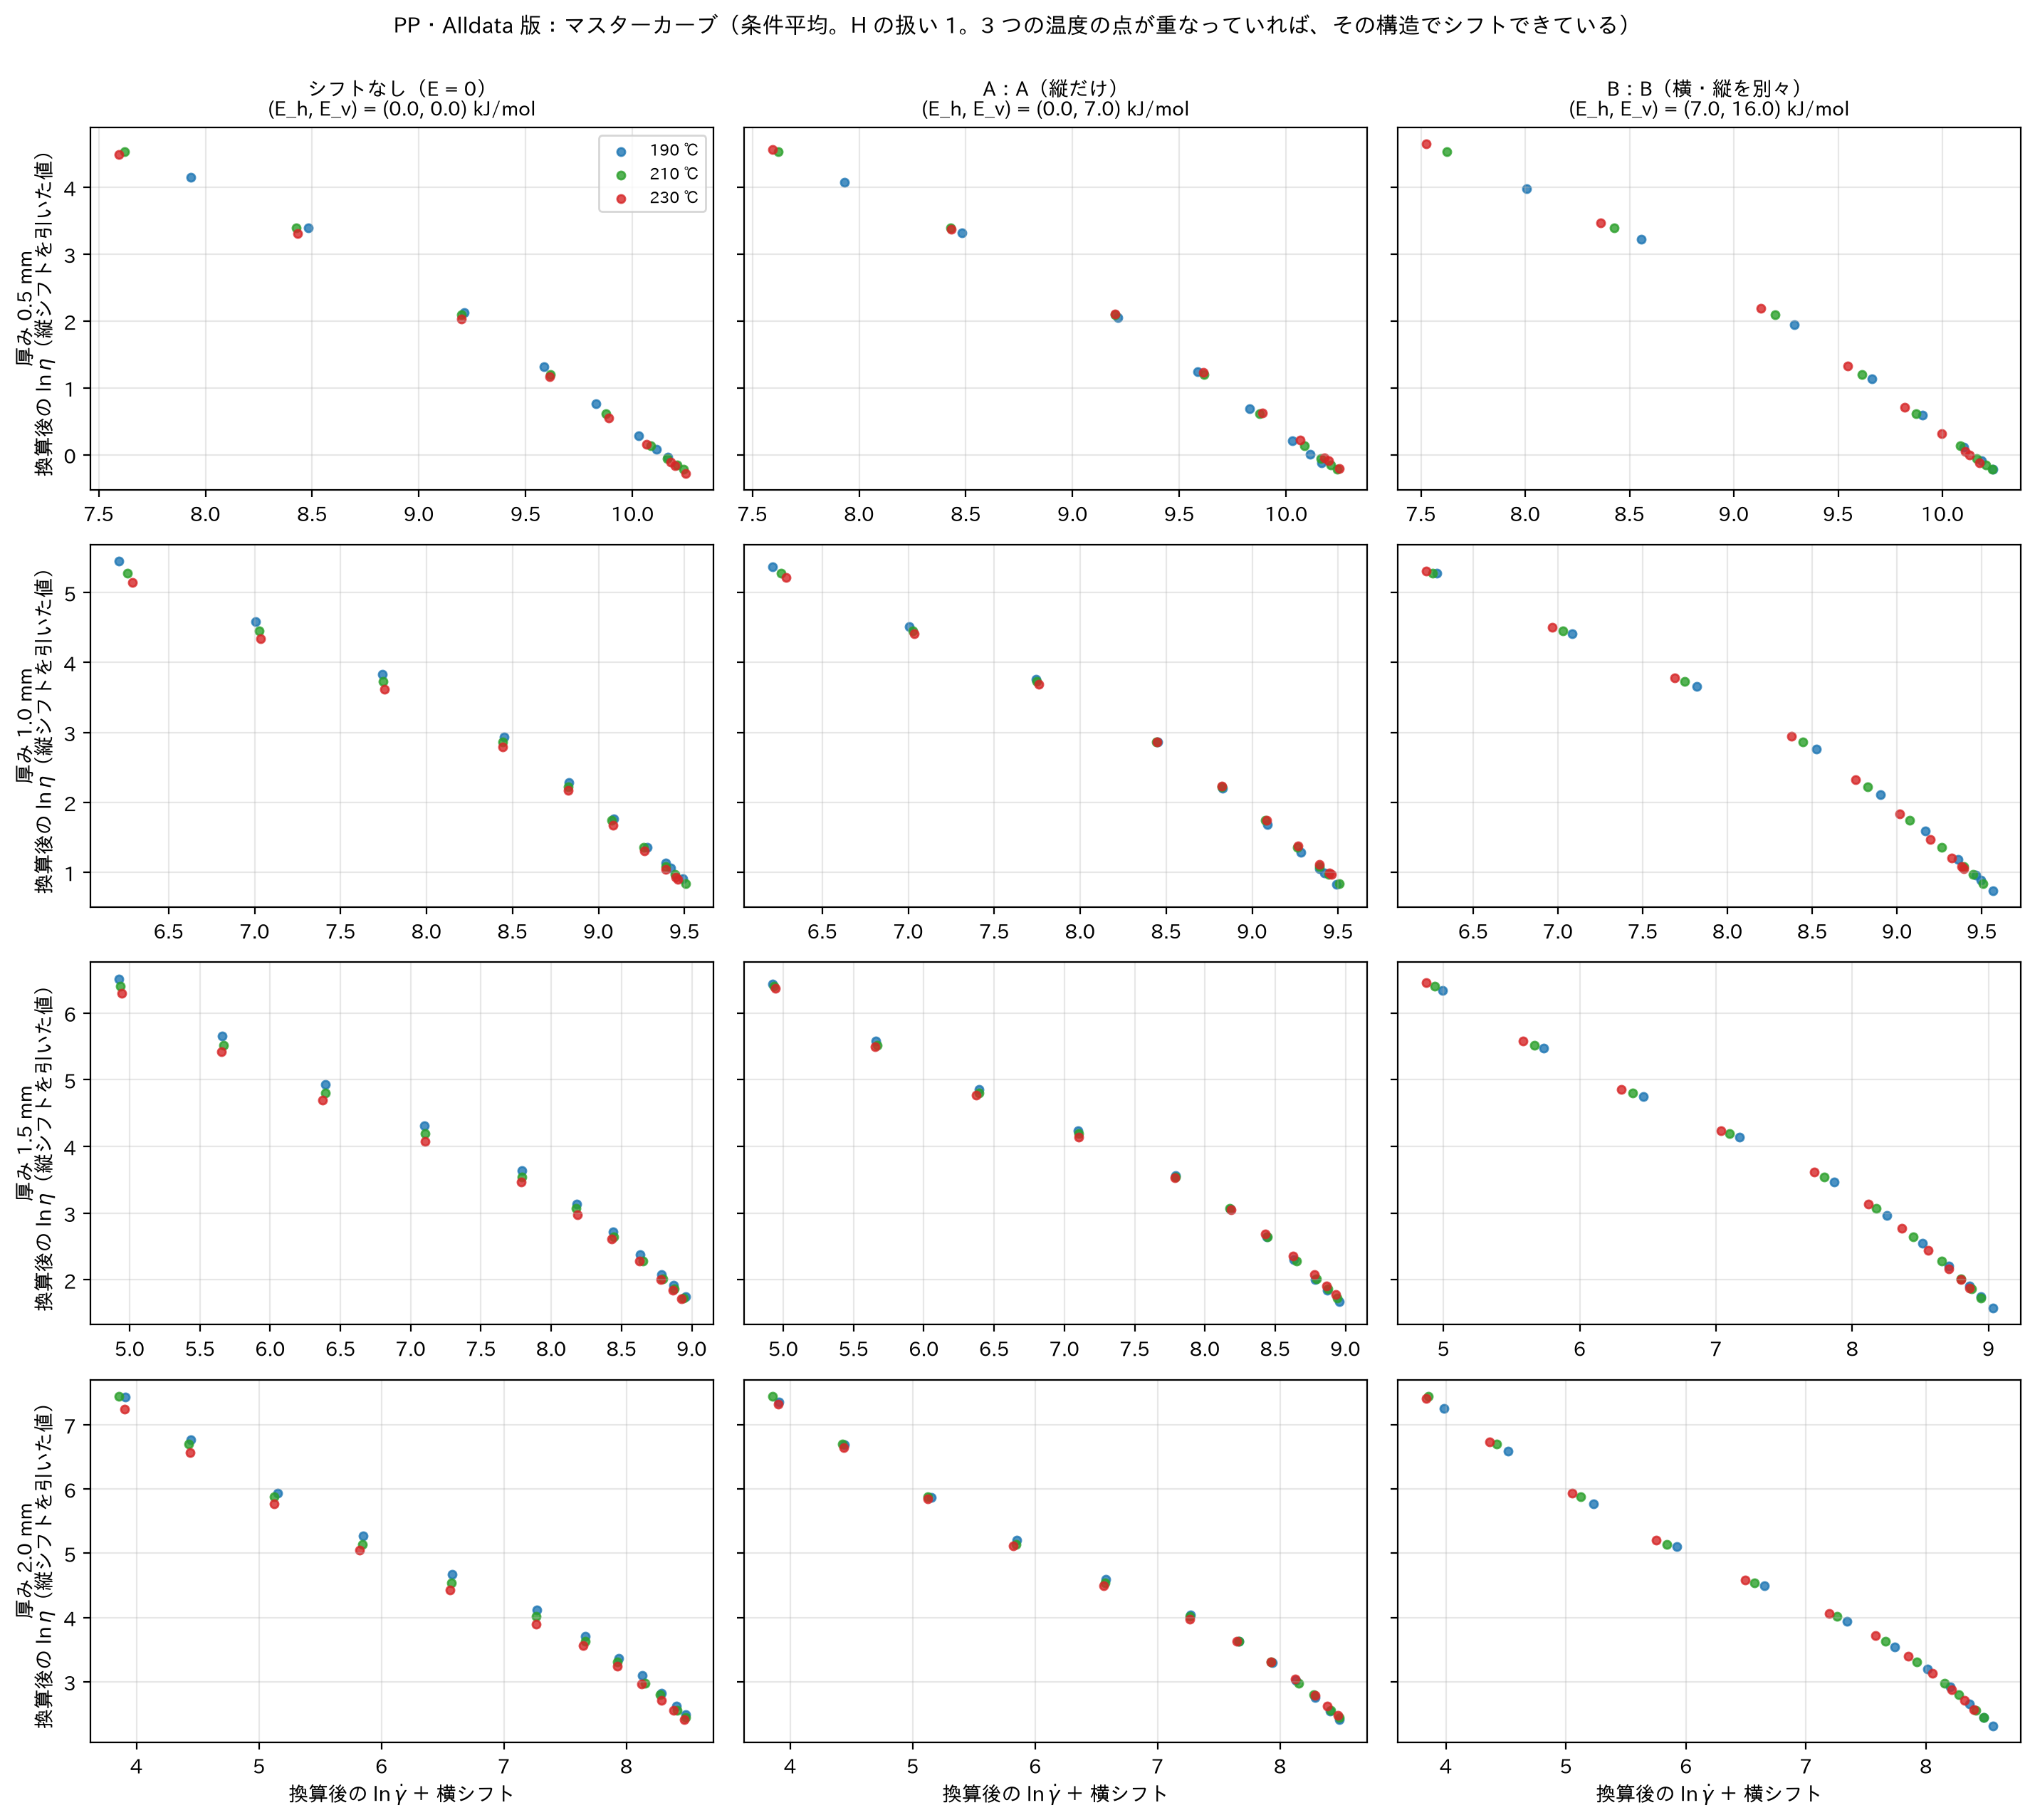
\includegraphics[width=0.97\linewidth]{fig3_master_Alldata_PP.png}
\caption{温度シフトで換算したあとの条件平均（行が厚み。左から：シフトなし、A、B。色が設定温度）}
\end{figure}
\begin{points}
\pt{何を示す図か}各条件の点（条件平均）を、温度シフトでずらしたあとの位置に描いた図です。シフトの目的は、3 つの温度の点を、1 本の曲線（マスターカーブ）に重ねることです。（ファイル：\file{fig3_master_Alldata_PP.png}。\file{highres/} に 600 dpi 版もあります）
\pt{軸と記号}横軸は換算後の $\ln\gd$（B は $\ln\gd+\ln a_T(\Eh)$）、縦軸は換算後の $\ln\eta$（縦シフトを引いた値）。青 190 ℃、緑 210 ℃、赤 230 ℃。
\pt{見るポイント}同じ厚みの中で、3 つの色の点が、1 本の曲線の上に重なっているか。
\pt{今回の結果}シフトなし（左）では、3 つの温度が、縦に少しずれて並びます（低温ほど上）。A（中）は、縦のずれを一定の倍率で消し、点がよく重なります。B（右）は、横にもずらすため、同じ厚みの中で、温度ごとに点が少し横にずれて並びますが、3 つの温度の点は、ほぼ 1 本の曲線の上にあります。A も B も、3 つの温度のデータを、1 本の曲線で表せることを示します。
\end{points}

\subsection{図4：設定温度ごとの予測曲線（PP・Alldata 版、H の扱い (1)）}
\begin{figure}[H]
\centering
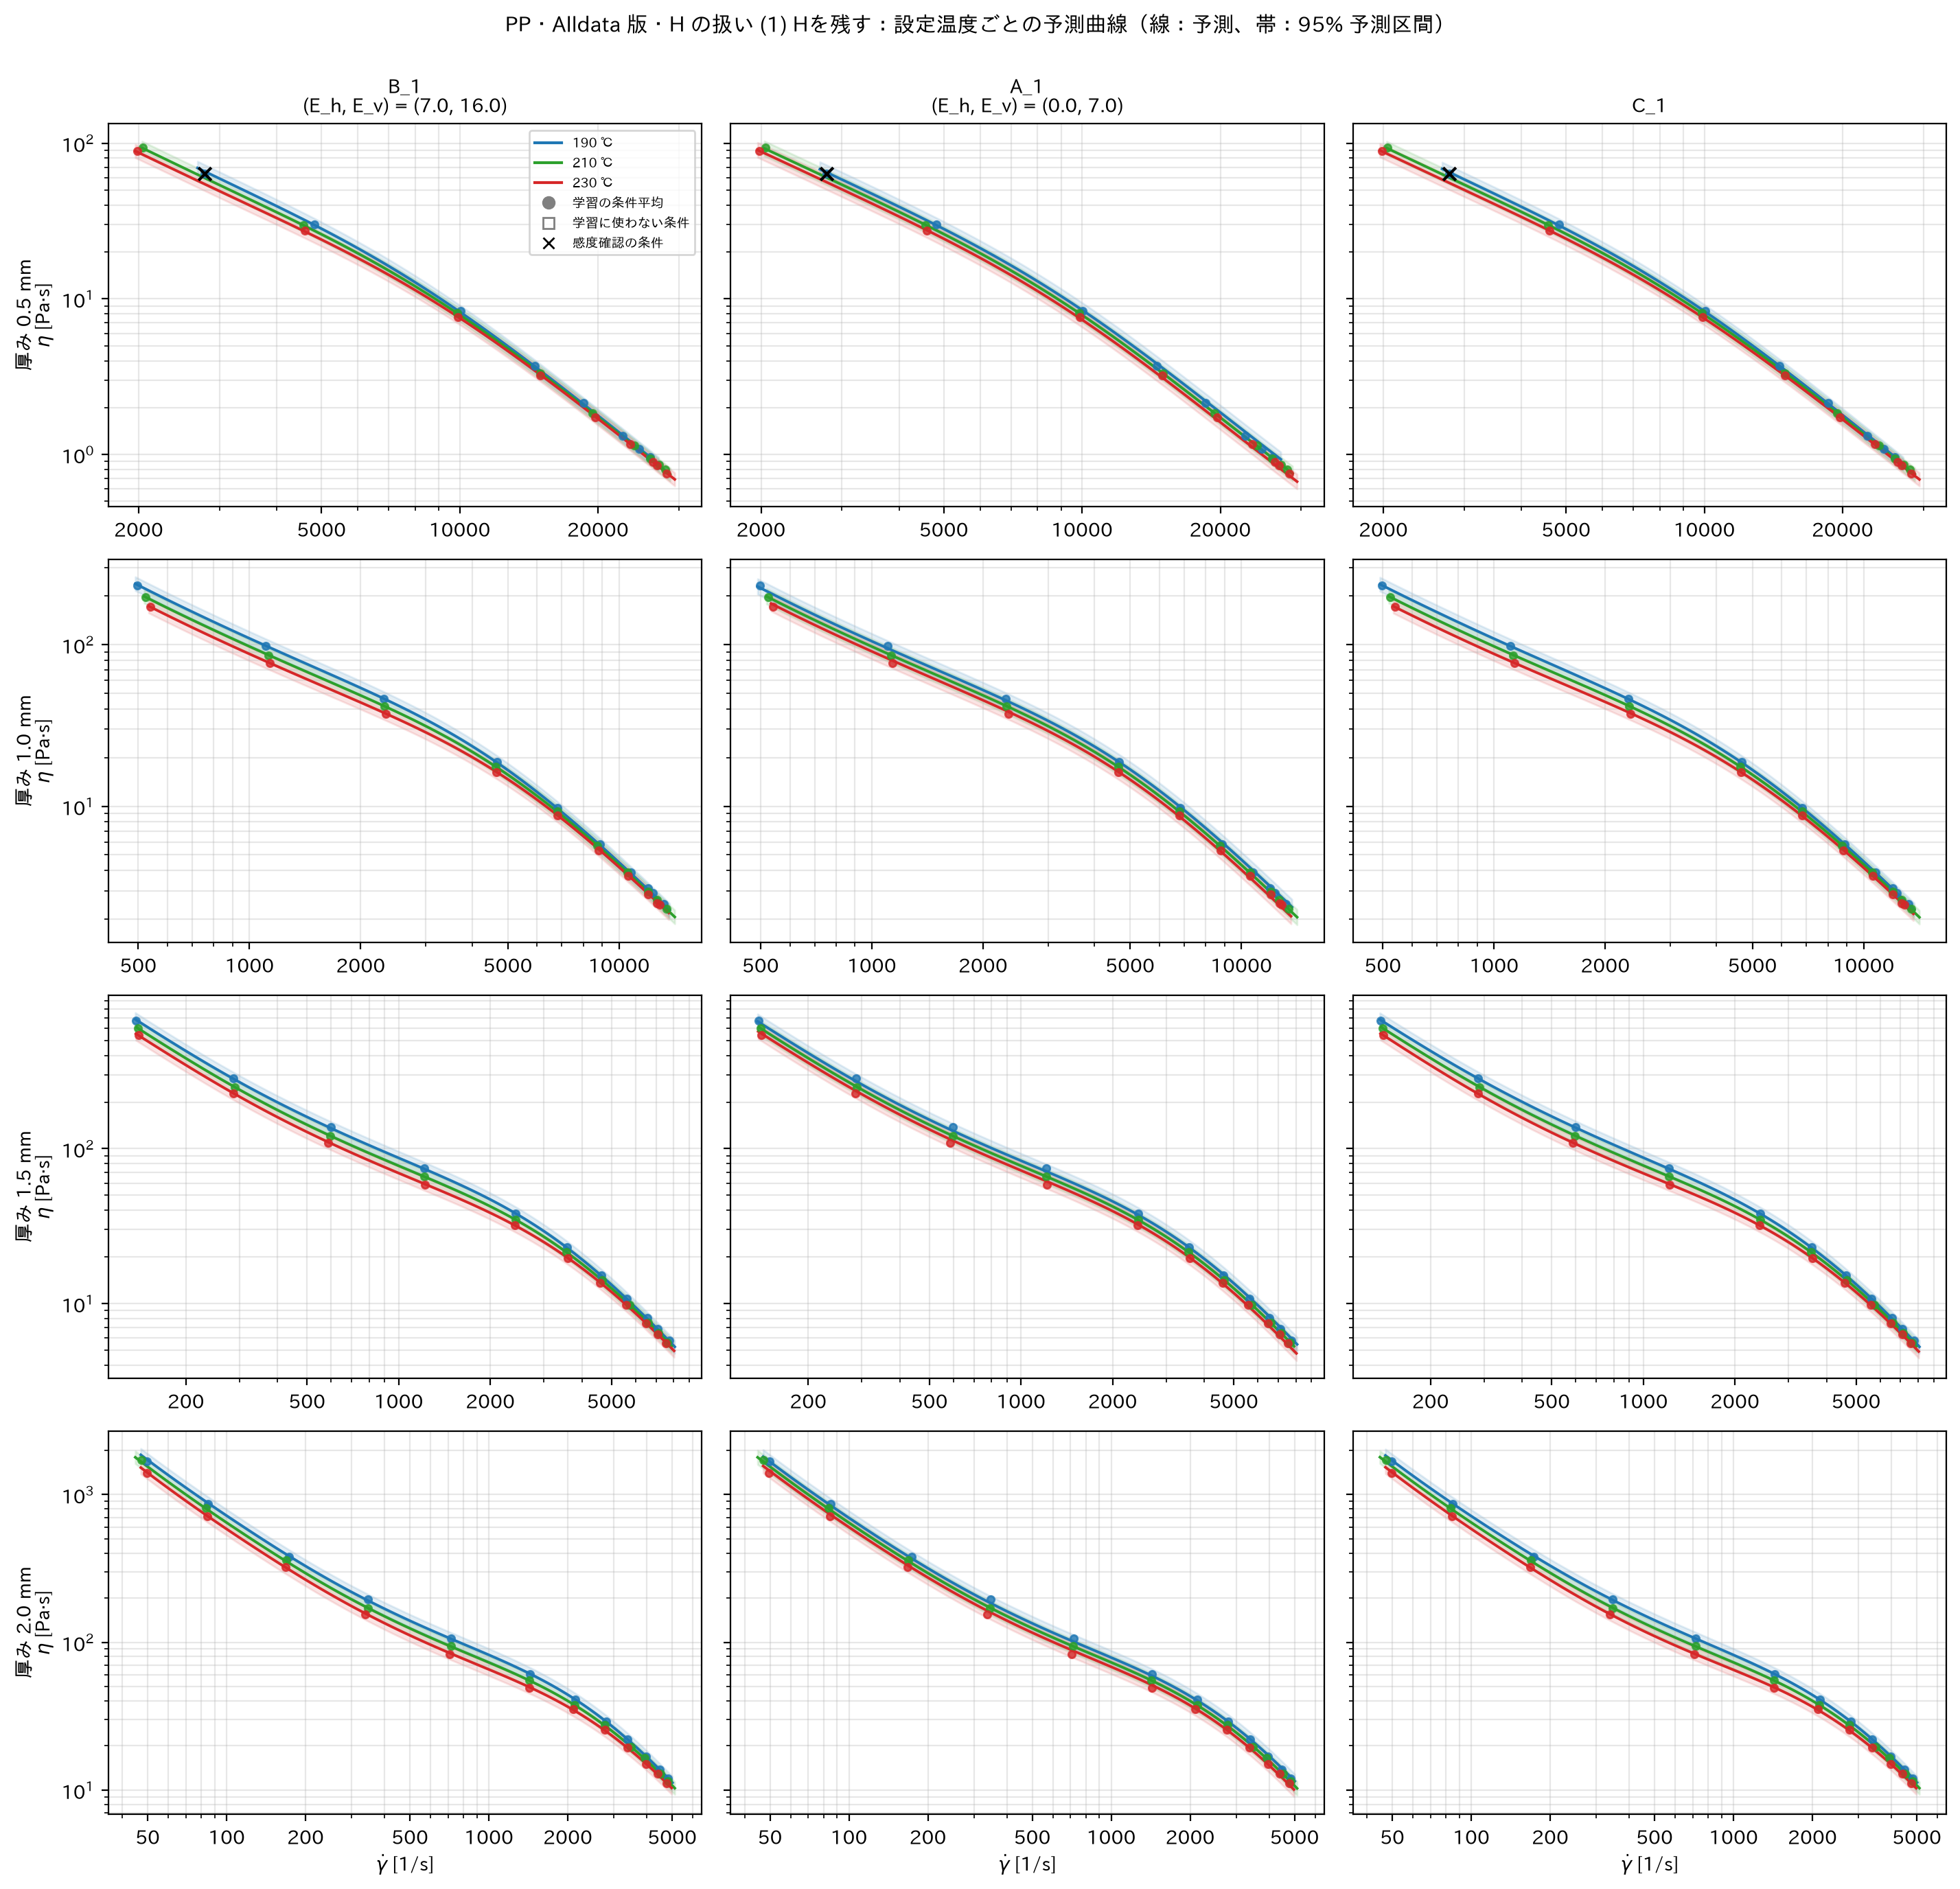
\includegraphics[width=0.95\linewidth]{fig4_curves_Alldata_PP_1.png}
\caption{予測曲線と 95\% 予測区間（行が厚み、列が構造 B・A・C。最終モデル。線の色が設定温度）}
\end{figure}
\begin{points}
\pt{何を示す図か}最終モデル（Alldata 全条件で学習）が、せん断速度と粘度の関係を、設定温度ごとにどう描くかを示した図です。（ファイル：\file{fig4_curves_Alldata_PP_1.png}。\file{highres/} に 600 dpi 版もあります）
\pt{軸と記号}横軸はせん断速度、縦軸は粘度（どちらも対数）。青 190 ℃・緑 210 ℃・赤 230 ℃。線が予測、薄い帯が 95\% 予測区間、点が学習の条件平均。$\times$ は問題データ一覧の「感度確認」の条件。(2)(4) の図は \file{fig4_curves_Alldata_PP_2.png}・\file{fig4_curves_Alldata_PP_4.png}（ほかの材料・版も同じ名前の形）。
\pt{見るポイント}点が帯の中に入っているか。3 つの温度の曲線の間隔（温度の効果）が、厚みやせん断速度でどう変わるか。
\pt{今回の結果}B・A・C のどれも、点が帯に入り、温度ごとの曲線が 190 ℃ > 210 ℃ > 230 ℃ の順に並びます。B と C は、厚いほど（また低せん断速度ほど）曲線の間隔が広がり、実測の「厚いほど温度の効果が大きい」傾向を表します。A は、どの厚みでも間隔が一定です。(4) を含む図では、P3\_2 を、同じ厚み・温度の条件平均から内挿して描いています（予測のときには分からない値です）。
\end{points}

\subsection{図5：評価指標の比較（Alldata 版）}
\begin{figure}[H]
\centering
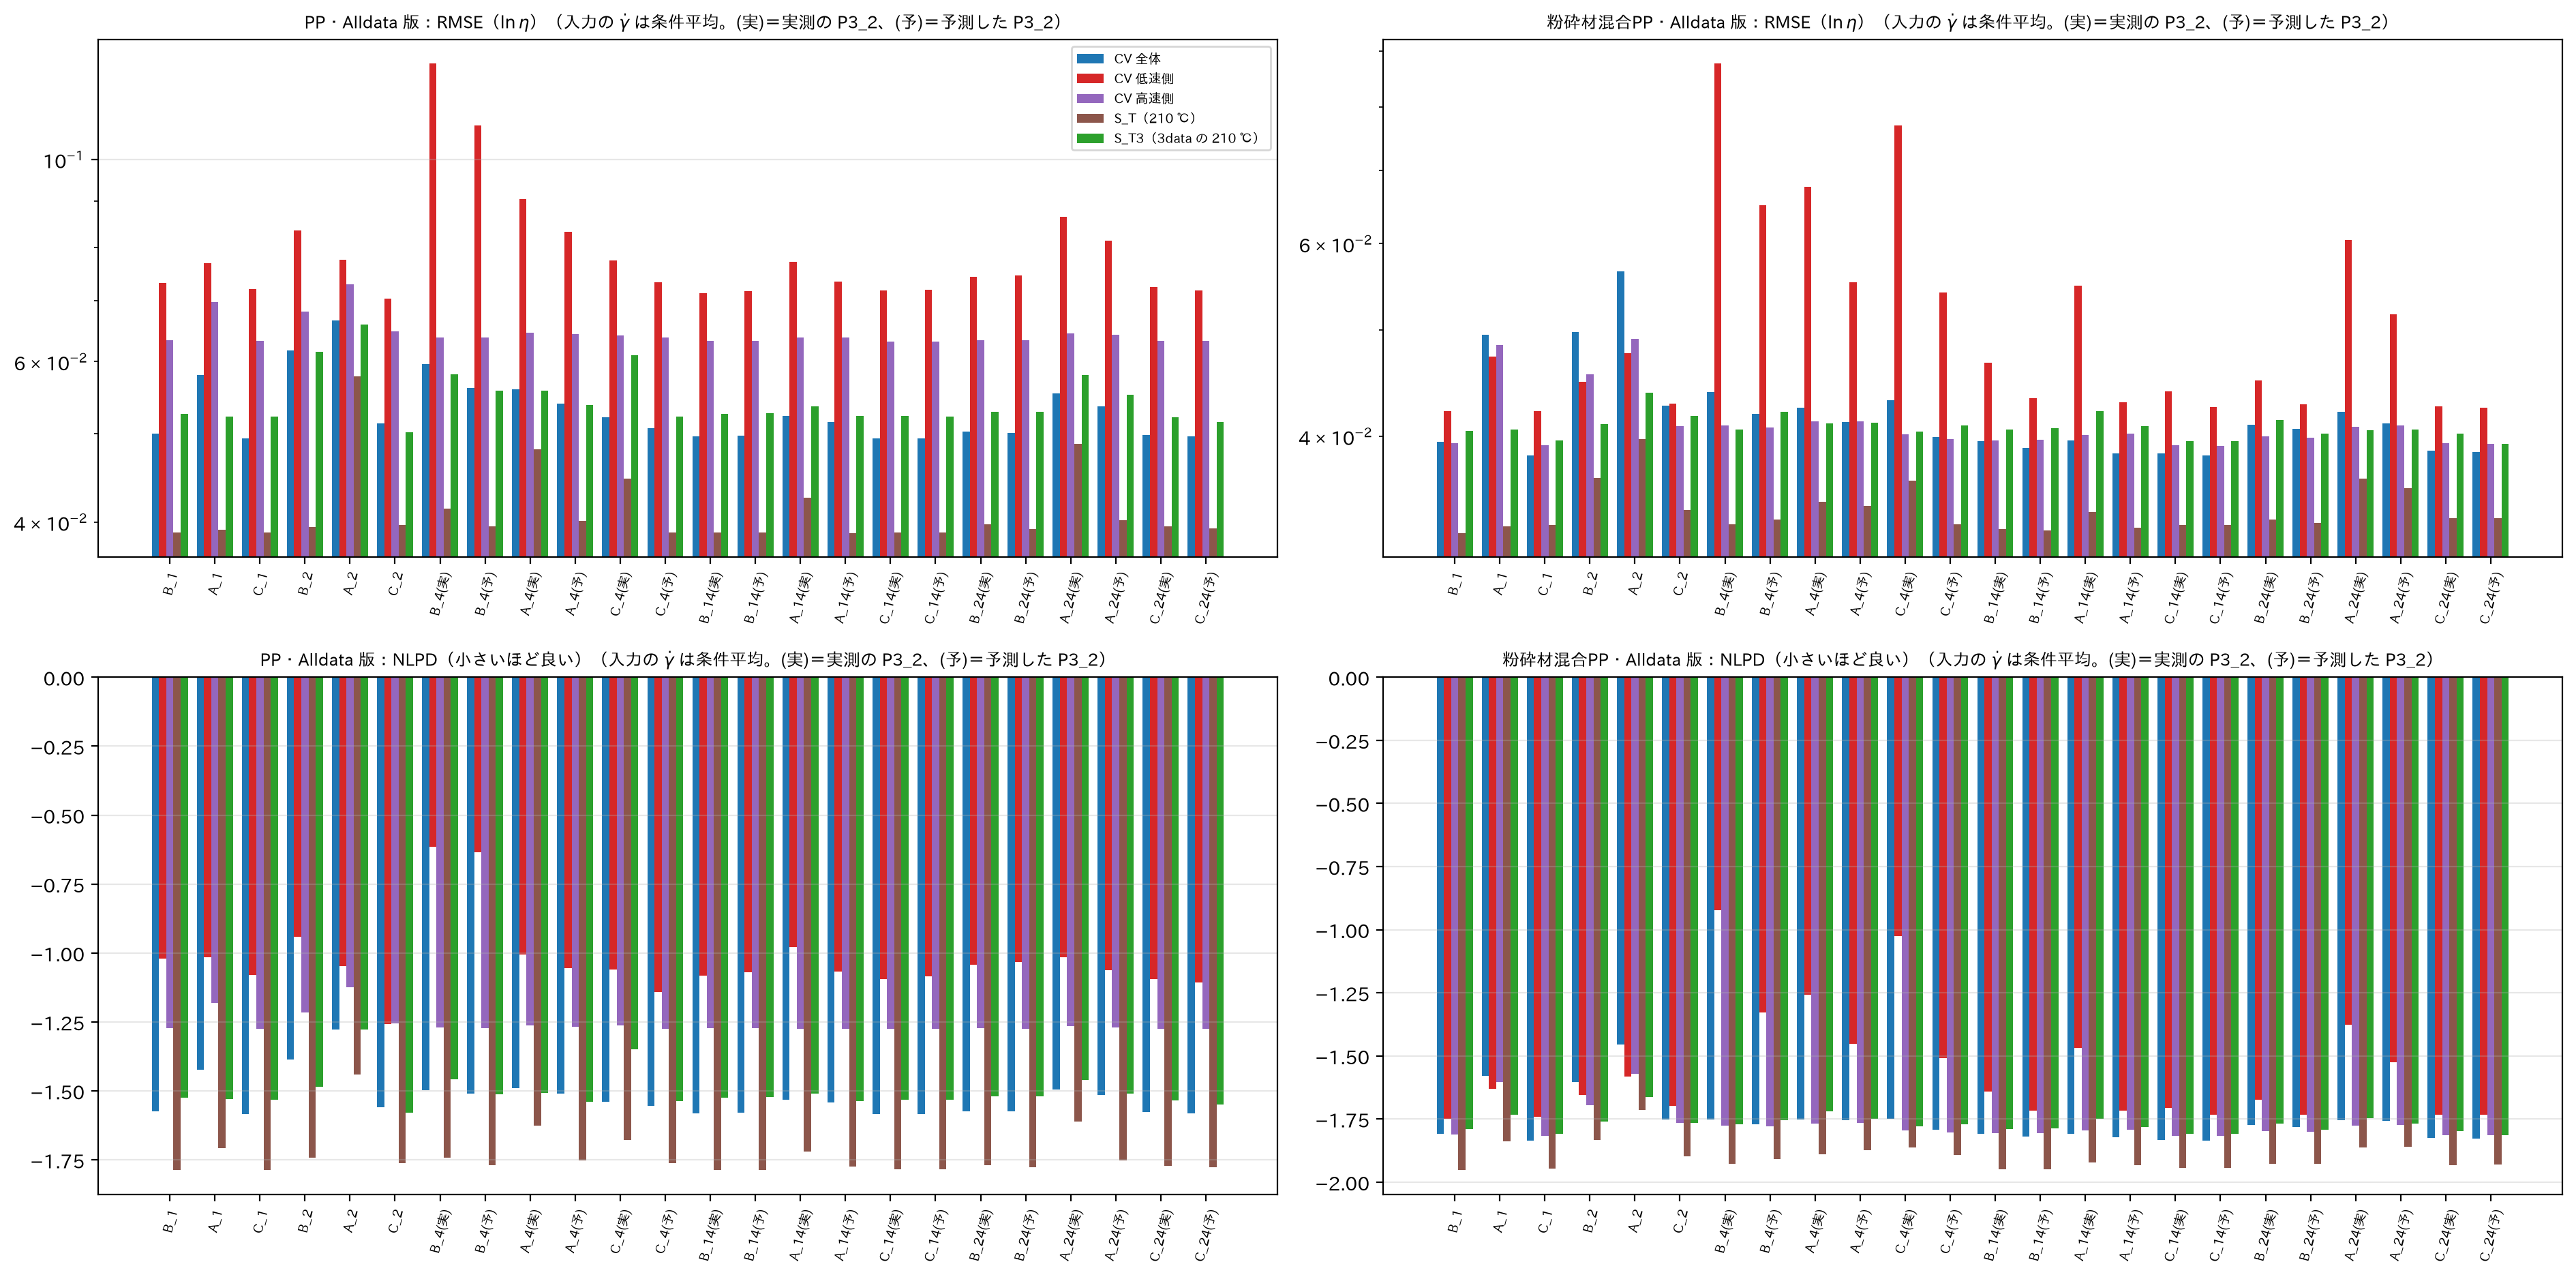
\includegraphics[width=1.0\linewidth]{fig5_metrics_Alldata.png}
\caption{15 モデルの RMSE と NLPD（左：PP、右：粉砕材混合 PP。色が検証の種類。(実)(予) は、実測／予測した P3\_2）}
\end{figure}
\begin{points}
\pt{何を示す図か}15 のモデルを、検証の種類ごとに、並べて比べた図です。（ファイル：\file{fig5_metrics_Alldata.png}。\file{highres/} に 600 dpi 版もあります）
\pt{軸と記号}横軸がモデル（構造\_扱い）、縦軸が RMSE（上段。対数軸）と NLPD（下段）。どちらも小さいほどよい。色は検証：青 CV 全体など（凡例参照）。
\pt{見るポイント}(1) の 3 本（B\_1・A\_1・C\_1）の高さがそろっているか。(2)・(4) で、特定の検証だけ高くならないか。
\pt{今回の結果}CV 全体では、B\_1 と C\_1 がほぼ同じで（PP：0.050 と 0.049。粉砕材混合 PP：0.040 と 0.038）、A\_1 はやや高く（0.058・0.050）なります。(2) は、CV 全体で (1) より $+$23\%（PP の B）高く、(4) の一部（B\_4 など）は、低速側の検証だけが高くなります。(1+4) は (1) と同じ高さです。5data 版の図（\file{fig5_metrics_5data.png}）では、外挿（S\_V 低速側）で、(2)(4) の高さが大きく違います（表\ref{tab:met_5data_PP}）。
\end{points}

\subsection{図6：設定温度の効果（Alldata 版）}
\begin{figure}[H]
\centering
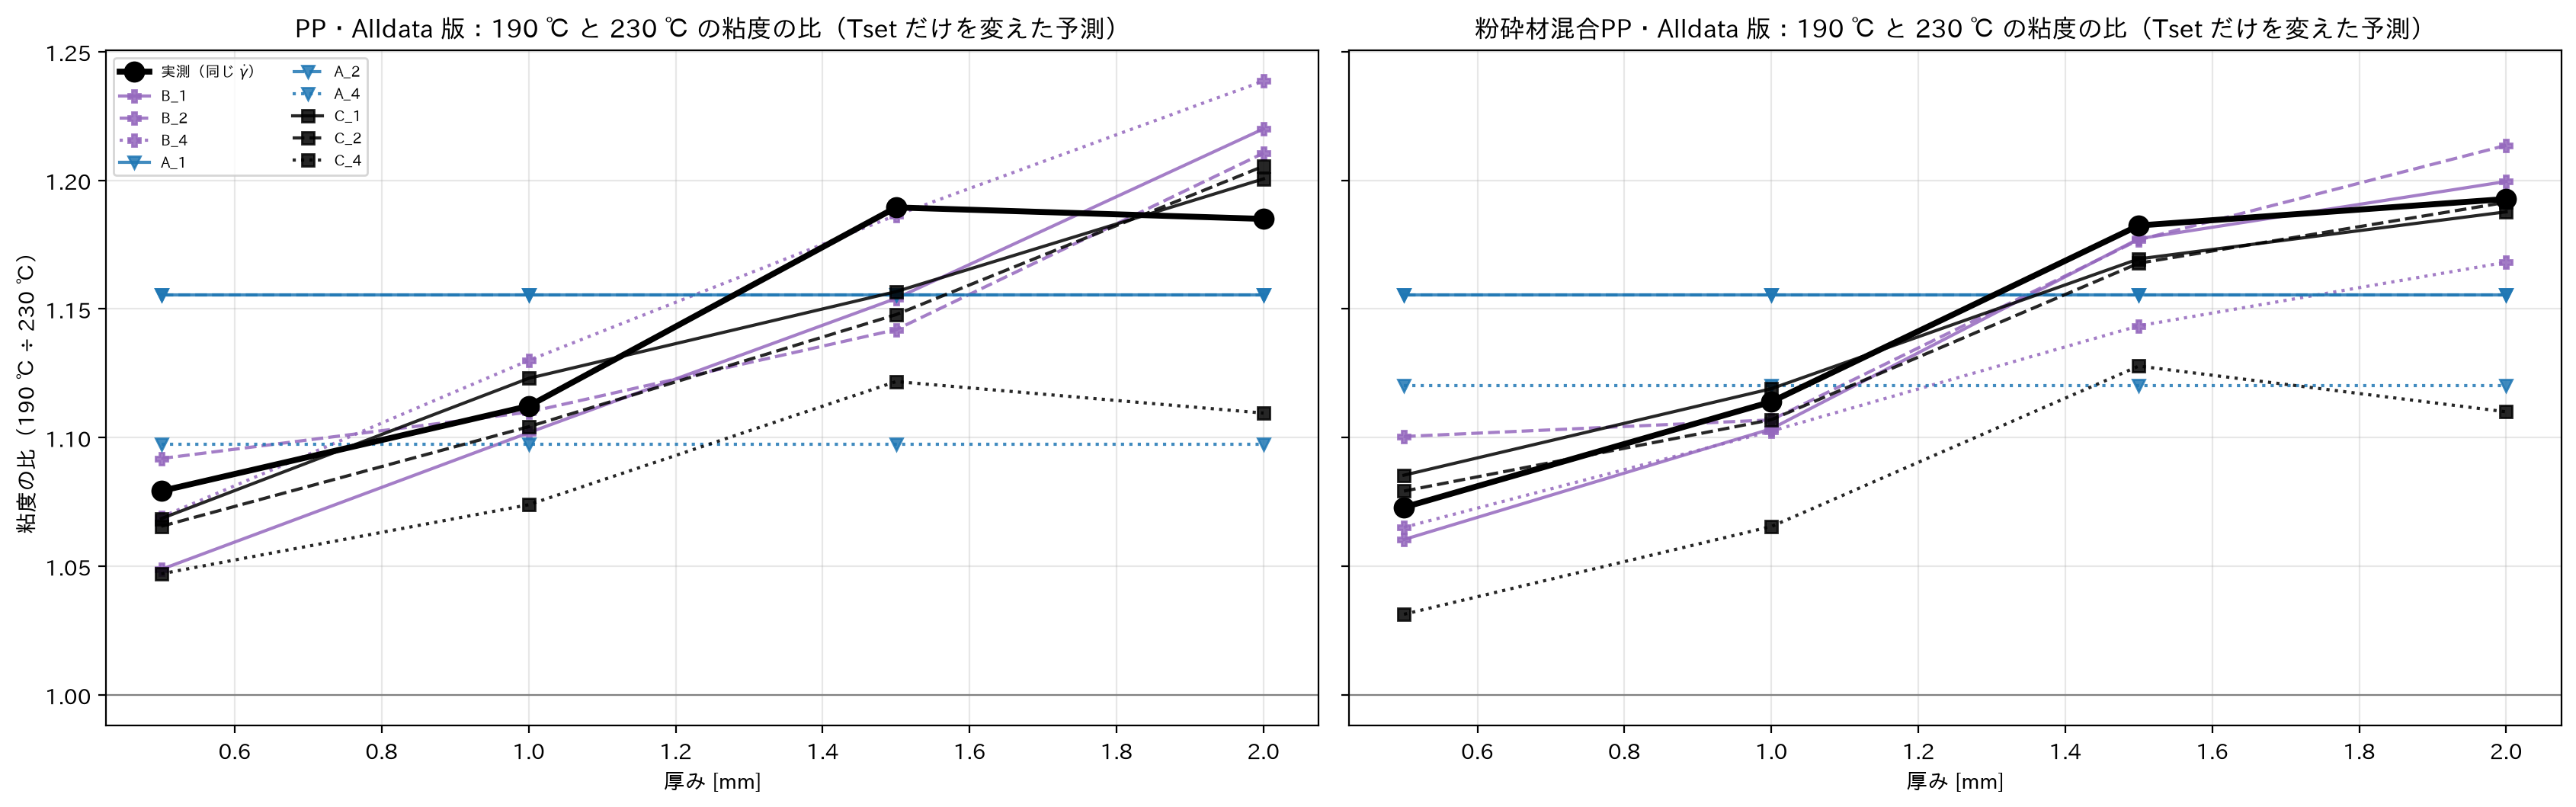
\includegraphics[width=0.97\linewidth]{fig6_tset_effect_Alldata.png}
\caption{190 ℃ と 230 ℃ の粘度の比（同じ $\gd$。厚みごと。太い黒線が実測、細い線が各モデルの予測）}
\end{figure}
\begin{points}
\pt{何を示す図か}Tset だけを 190 ℃ から 230 ℃ に変えたときの粘度の比を、厚みごとに、実測と各モデルで比べた図です。（ファイル：\file{fig6_tset_effect_Alldata.png}。\file{highres/} に 600 dpi 版もあります）
\pt{軸と記号}横軸は厚み [mm]、縦軸は粘度の比（190 ℃ の粘度 ÷ 230 ℃ の粘度）。太い黒線が実測。線の色は構造（紫 B、青 A、黒 C）、線の種類は $H$ の扱い（実線 (1)、破線 (2)、点線 (4)）。
\pt{見るポイント}実測の傾向（厚いほど比が大きい）を、モデルが表せているか。
\pt{今回の結果}実測の比は、厚み 0.5 → 2.0 mm で、PP 1.08 → 1.19 と、厚いほど大きくなります。B\_1・C\_1 は、この傾向をよく表します（PP の B\_1：1.05 → 1.22）。A は、構造上、どの厚みでも一定（約 1.16）で、傾向を表せません。(4) の C\_4 は、傾向が弱く、1.5 mm 以上で頭打ちになります（表\ref{tab:tset}）。
\end{points}

\subsection{図7：(2) の分解 ―― 材料の部分 $m$ と、厚み・冷却の補正 $c$（PP・Alldata 版）}
\begin{figure}[H]
\centering
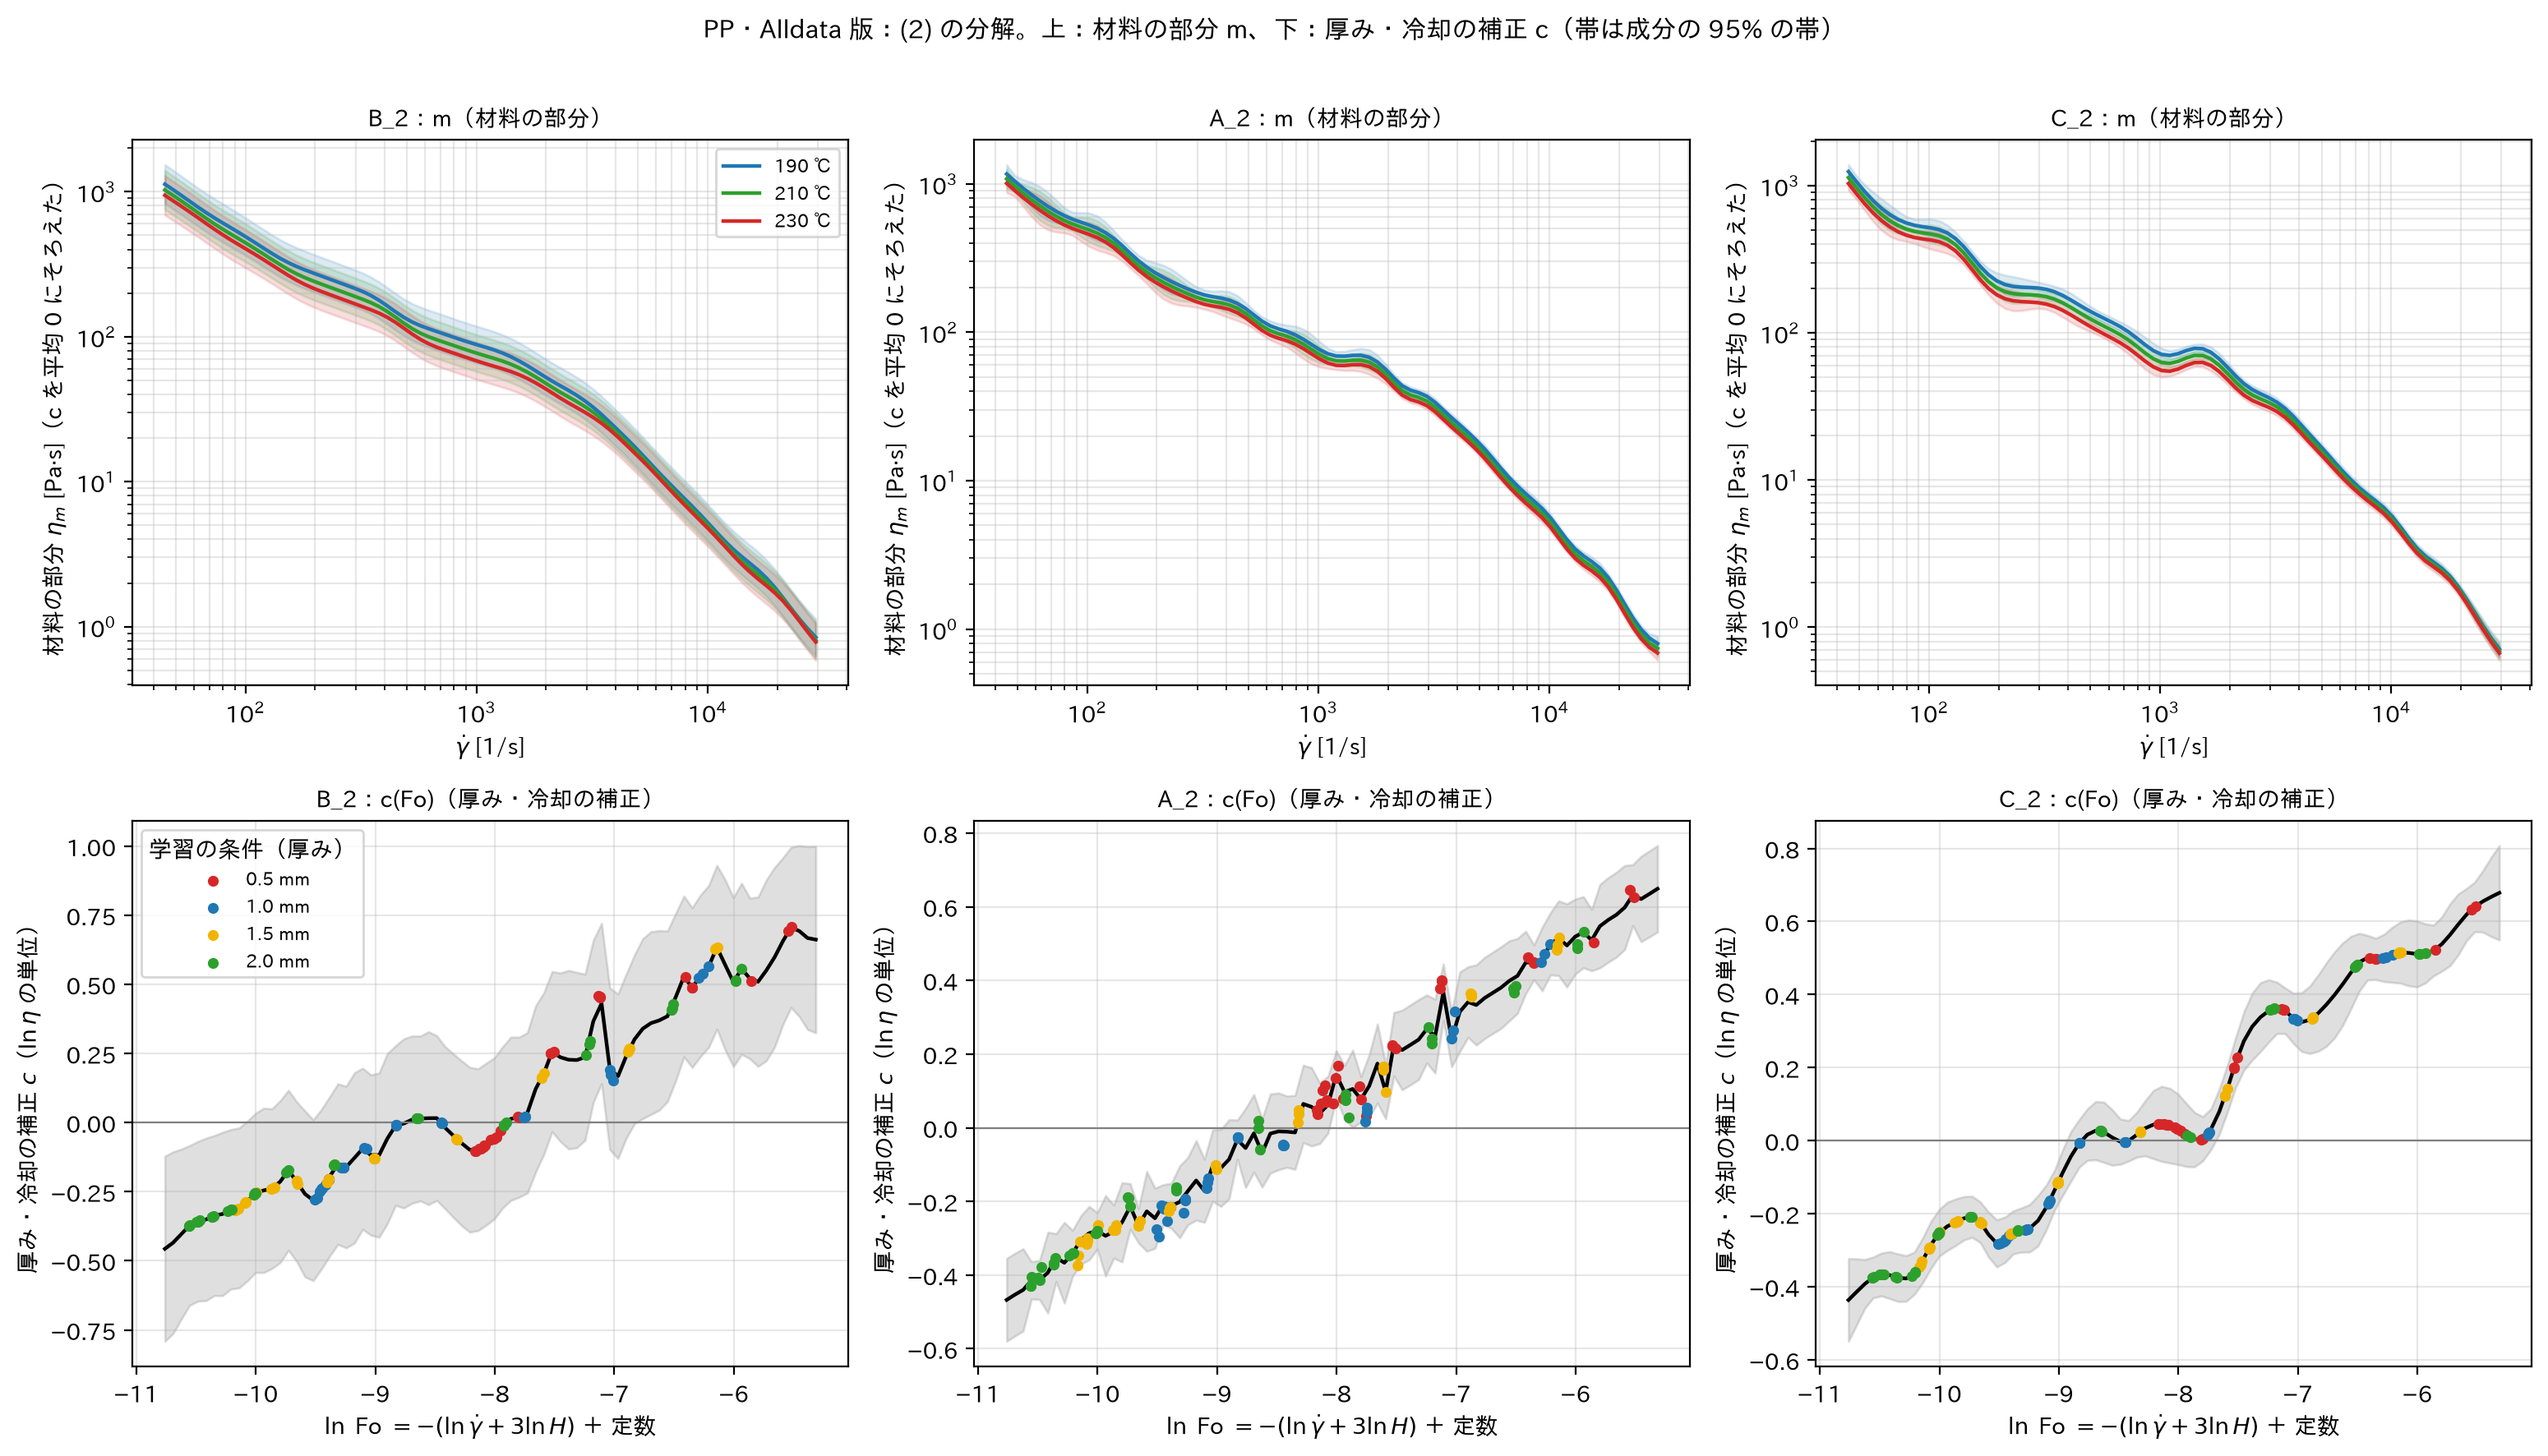
\includegraphics[width=0.97\linewidth]{fig7_decomposition_Alldata_PP.png}
\caption{上：$m$（材料の部分。設定温度ごと）、下：$c$（ln Fo の関数。点は学習の条件、色は厚み）。列は構造 B・A・C}
\end{figure}
\begin{points}
\pt{何を示す図か}H の扱い (2)（$m$ と $c$ の足し算）の最終モデルを、2 つの成分に分けて見せた図です。（ファイル：\file{fig7_decomposition_Alldata_PP.png}。\file{highres/} に 600 dpi 版もあります）
\pt{軸と記号}上段：横軸は $\gd$、縦軸は材料の部分の粘度（$c$ の平均を 0 にそろえたもの）。3 本の線が設定温度。下段：横軸は $\ln\mathrm{Fo}=-(\ln\gd+3\ln H)$ ＋ 定数、縦軸は厚み・冷却の補正 $c$（$\ln\eta$ の単位）。灰色の帯が 95\% の帯。
\pt{見るポイント}上段が、せん断速度とともに下がる滑らかな曲線（Cross-WLF の粘度曲線のような形）で、温度で位置が変わるか。下段の補正 $c$ が、どれくらいの大きさか。
\pt{今回の結果}材料の部分 $m$ は、滑らかな右下がりの曲線で、温度で上下します（B は横にもずれます）。補正 $c$ は、$\ln\mathrm{Fo}$ とともにほぼ直線的に増え、最大と最小の差が約 1.1（粘度で約 3 倍）あり、温度の効果（$\ln$ で 0.17 ほど）よりはるかに大きい補正です。つまり、「見かけの粘度」の変化の大部分は、冷却・固化に由来する厚みの補正が占めています（表\ref{tab:dec}）。
\end{points}

\subsection{図8：P3\_2 の予測（5data 版）}
\begin{figure}[H]
\centering
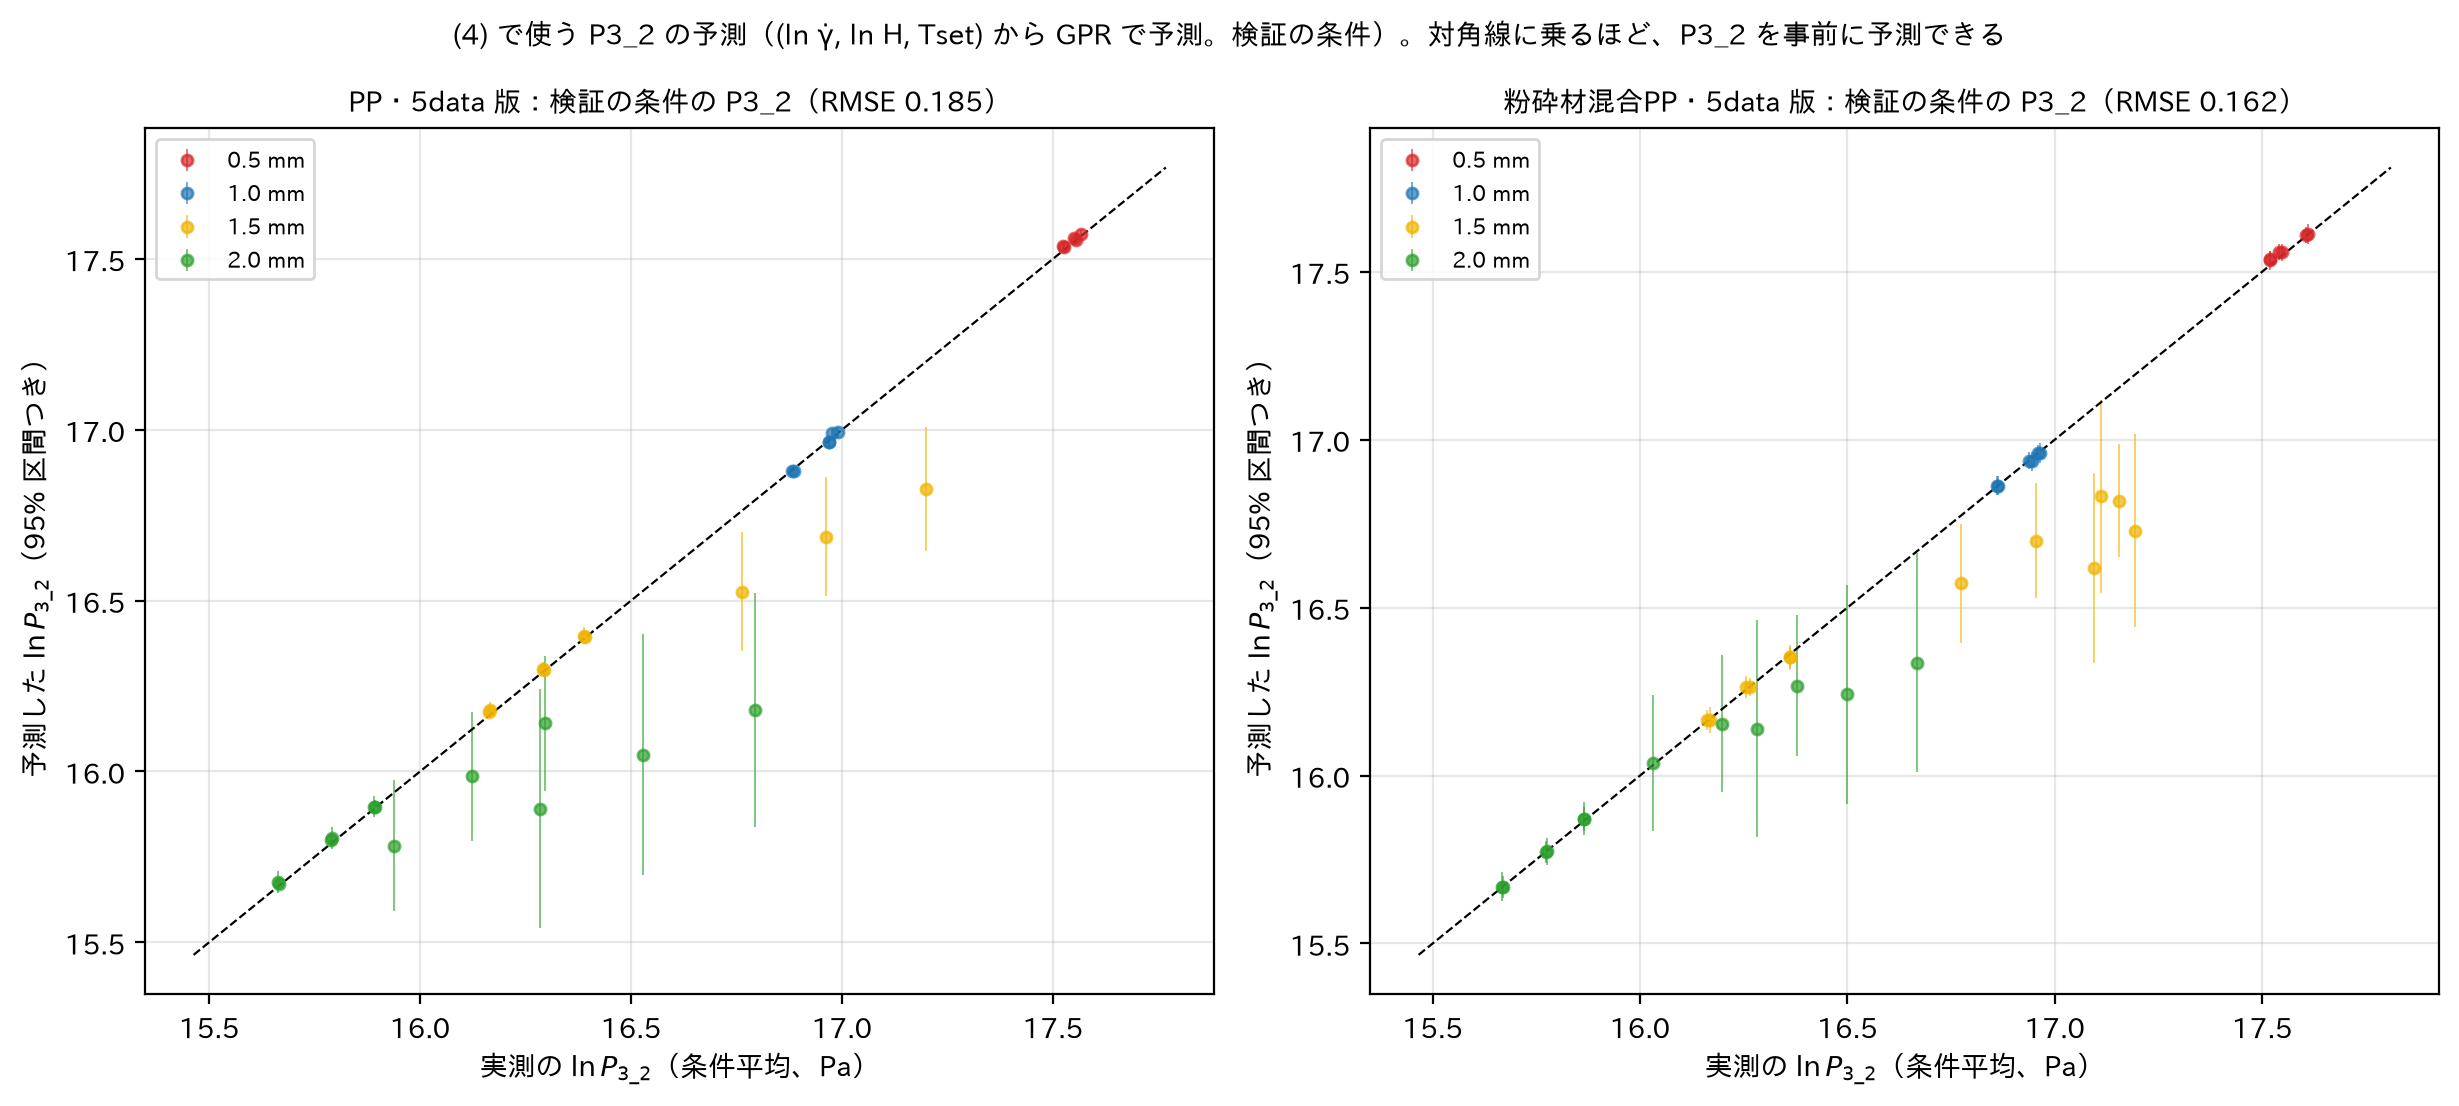
\includegraphics[width=0.97\linewidth]{fig8_p32_pred_5data.png}
\caption{(4) で使う P3\_2 の、実測と予測（検証の条件。縦棒は 95\% 区間。色は厚み）}
\end{figure}
\begin{points}
\pt{何を示す図か}(4) の「予測した P3\_2」を作るモデル（$(\ln\gd,\ln H,\Tset)$ から $\ln$ P3\_2 を予測する GPR）が、検証の条件の P3\_2 を、どれだけ当てられるかを示した図です。（ファイル：\file{fig8_p32_pred_5data.png}。\file{highres/} に 600 dpi 版もあります）
\pt{軸と記号}横軸が実測の $\ln$ P3\_2（条件平均、Pa）、縦軸が予測。黒い破線が一致の線（対角線）。点の色が厚み。
\pt{見るポイント}点が対角線の近くにあるか。外れる点は、どの厚み・条件か。
\pt{今回の結果}点はほぼ対角線に乗り、ln P3\_2 の予測の RMSE は、5data 版の外挿で PP 0.19、Alldata 版の CV で 0.024 と小さいです（粘度の ln η の誤差は 0.05 ほど）。外れるのは、外挿側の 1.5〜2.0 mm の厚い条件（予測が低め）です。つまり、\PII\ は、$H$・$\gd$・$\Tset$ から、ほぼ予測できます。\PII\ が厚みの情報を持つ（$H$ の代わりの目印）、手順3e の結論と一致します。
\end{points}


% =====================================================================
\section{表の見方}


\subsection{表\ref{tab:E}：最良の $E$}
\begin{table}[H]
\caption{構造 A・B の最良の $E$（kJ/mol）。5data 版は S\_V の学習、Alldata 版は ALL の学習。差＝$\Ev-\Eh$（括弧：LML が最大から 1.92 以内の範囲）。ΔLML＝B の LML $-$ A の LML（同じ $H$ の扱い）}\label{tab:E}
\footnotesize
\begin{tabularx}{\linewidth}{@{}llllllXr@{}}
\toprule
材料 & 版 & 扱い & A の $\Ev$ & B の $\Eh$ & B の $\Ev$ & 差（範囲） & ΔLML \\
\midrule
PP & 5data & (1) & 7.5 & 6 & 15 & 9（9〜9） & 78 \\
 &  & (2) & 7.5 & 4 & 12 & 8（8〜8） & 38 \\
 &  & (4) & 5.0 & 6 & 17 & 11（10〜11） & 29 \\
 &  & (1+4) & 5.0 & 6 & 15 & 9（9〜9） & 52 \\
 &  & (2+4) & 5.0 & 7 & 17 & 10（10〜10） & 65 \\
\midrule
粉砕材混合 PP & 5data & (1) & 7.5 & 7 & 16 & 9（9〜9） & 52 \\
 &  & (2) & 7.5 & 4 & 12 & 8（8〜8） & 28 \\
 &  & (4) & 5.0 & 2 & 8 & 6（6〜7） & 9 \\
 &  & (1+4) & 5.0 & 2 & 8 & 6（6〜6） & 9 \\
 &  & (2+4) & 5.0 & 7 & 17 & 10（9〜10） & 25 \\
\midrule
PP & Alldata & (1) & 7.0 & 7 & 16 & 9（9〜9） & 114 \\
 &  & (2) & 7.0 & 7 & 16 & 9（9〜9） & 43 \\
 &  & (4) & 4.5 & 6 & 17 & 11（11〜11） & 52 \\
 &  & (1+4) & 5.0 & 6 & 15 & 9（9〜9） & 79 \\
 &  & (2+4) & 4.5 & 7 & 17 & 10（10〜10） & 98 \\
\midrule
粉砕材混合 PP & Alldata & (1) & 7.0 & 7 & 16 & 9（9〜9） & 81 \\
 &  & (2) & 7.0 & 7 & 16 & 9（9〜9） & 32 \\
 &  & (4) & 5.5 & 4 & 12 & 8（8〜8） & 18 \\
 &  & (1+4) & 5.5 & 2 & 9 & 7（6〜7） & 14 \\
 &  & (2+4) & 5.5 & 6 & 15 & 9（9〜9） & 42 \\

\bottomrule
\end{tabularx}
\end{table}
\begin{points}
\pt{読み方}A の $\Ev$ は 7〜7.5 kJ/mol（$H$ を残すとき）。B は $(\Eh,\Ev)\approx(6\text{〜}7,\ 15\text{〜}16)$、差は約 9。B の LML が A より大きい（ΔLML は PP の Alldata 版 (1) で 114）ので、「横のシフトも必要」とデータが言っています。\PII\ を入れる扱い (4)(1+4)(2+4) では、A の $\Ev$ が 4.5〜5.5 に小さくなり、B の $\Eh$・$\Ev$ も少し動きます（\PII\ が、温度による粘度の違いの一部を持つため）。CV の 10 分割でも、A の $\Ev$ のばらつき（標準偏差）は 0.2〜0.4、B の差は 0〜1.3 kJ/mol でした。
\end{points}

\subsection{表\ref{tab:met_5data_PP} ほか：検証の RMSE}
\begin{points}
\pt{表の種類}5data 版と Alldata 版、PP と粉砕材混合 PP の 4 つの表です。行が 15 モデル（構造 B・A・C $\times$ 扱い 5 通り）、列が検証の種類です。5data 版の S\_V は外挿（低速側・高速側）、S\_T は 210 ℃、S\_T3 は 3data の 210 ℃（速度の外挿も重なる）。Alldata 版の CV は、条件単位の 10 分割です。
\pt{(4) を含む行}「実測の \PII\ のときの値（予測した \PII\ のときの値）」の形で 2 つの値を書きました。
\end{points}
\begin{table}[H]
\caption{PP・5data 版（学習 5data）：RMSE（$\ln\eta$）。(4) を含む行は、実測の \PII\ のとき（括弧の中が、予測した \PII\ のとき）}\label{tab:met_5data_PP}
\footnotesize
\begin{tabularx}{\linewidth}{@{}llXXXX@{}}
\toprule
扱い & モデル & S\_V 低速側 & S\_V 高速側 & S\_T & S\_T3 \\
\midrule
(1) & B\_1 & 0.073 & 0.053 & 0.039 & 0.051 \\
 & A\_1 & 0.057 & 0.062 & 0.040 & 0.069 \\
 & C\_1 & 0.064 & 0.053 & 0.039 & 0.060 \\
\midrule
(2) & B\_2 & 0.215 & 0.063 & 0.040 & 0.124 \\
 & A\_2 & 0.378 & 0.074 & 0.049 & 0.163 \\
 & C\_2 & 0.329 & 0.065 & 0.040 & 0.118 \\
\midrule
(4) & B\_4 & 0.157（0.077） & 0.056（0.056） & 0.044（0.039） & 0.058（0.070） \\
 & A\_4 & 0.162（0.075） & 0.059（0.060） & 0.048（0.041） & 0.070（0.056） \\
 & C\_4 & 0.141（0.072） & 0.054（0.054） & 0.045（0.039） & 0.063（0.080） \\
\midrule
(1+4) & B\_14 & 0.075（0.069） & 0.053（0.053） & 0.039（0.039） & 0.086（0.090） \\
 & A\_14 & 0.198（0.126） & 0.054（0.054） & 0.042（0.039） & 0.084（0.053） \\
 & C\_14 & 0.059（0.059） & 0.053（0.053） & 0.039（0.039） & 0.072（0.071） \\
\midrule
(2+4) & B\_24 & 0.128（0.126） & 0.053（0.053） & 0.040（0.039） & 0.050（0.051） \\
 & A\_24 & 0.164（0.083） & 0.056（0.056） & 0.048（0.040） & 0.071（0.064） \\
 & C\_24 & 0.120（0.119） & 0.053（0.053） & 0.040（0.040） & 0.123（0.117） \\
\multicolumn{2}{l}{純粋誤差（参考）} & \multicolumn{4}{l}{約 0.041} \\
\bottomrule
\end{tabularx}
\end{table}

\begin{table}[H]
\caption{粉砕材混合 PP・5data 版（学習 5data）：RMSE（$\ln\eta$）。(4) を含む行は、実測の \PII\ のとき（括弧の中が、予測した \PII\ のとき）}\label{tab:met_5data_MIX}
\footnotesize
\begin{tabularx}{\linewidth}{@{}llXXXX@{}}
\toprule
扱い & モデル & S\_V 低速側 & S\_V 高速側 & S\_T & S\_T3 \\
\midrule
(1) & B\_1 & 0.040 & 0.040 & 0.033 & 0.041 \\
 & A\_1 & 0.074 & 0.050 & 0.033 & 0.046 \\
 & C\_1 & 0.051 & 0.039 & 0.033 & 0.043 \\
\midrule
(2) & B\_2 & 0.208 & 0.059 & 0.038 & 0.124 \\
 & A\_2 & 0.338 & 0.063 & 0.046 & 0.187 \\
 & C\_2 & 0.255 & 0.052 & 0.034 & 0.142 \\
\midrule
(4) & B\_4 & 0.154（0.071） & 0.042（0.042） & 0.033（0.034） & 0.052（0.059） \\
 & A\_4 & 0.206（0.084） & 0.043（0.043） & 0.034（0.035） & 0.076（0.048） \\
 & C\_4 & 0.131（0.080） & 0.040（0.040） & 0.037（0.034） & 0.059（0.058） \\
\midrule
(1+4) & B\_14 & 0.089（0.192） & 0.040（0.040） & 0.033（0.033） & 0.056（0.098） \\
 & A\_14 & 0.110（0.222） & 0.040（0.040） & 0.033（0.033） & 0.080（0.144） \\
 & C\_14 & 0.159（0.177） & 0.039（0.039） & 0.033（0.033） & 0.092（0.103） \\
\midrule
(2+4) & B\_24 & 0.184（0.173） & 0.039（0.039） & 0.034（0.033） & 0.088（0.087） \\
 & A\_24 & 0.197（0.074） & 0.042（0.042） & 0.035（0.036） & 0.071（0.044） \\
 & C\_24 & 0.075（0.071） & 0.039（0.039） & 0.033（0.033） & 0.040（0.040） \\
\multicolumn{2}{l}{純粋誤差（参考）} & \multicolumn{4}{l}{約 0.039} \\
\bottomrule
\end{tabularx}
\end{table}

\begin{table}[H]
\caption{PP・Alldata 版（学習 Alldata）：RMSE（$\ln\eta$）。(4) を含む行は、実測の \PII\ のとき（括弧の中が、予測した \PII\ のとき）}\label{tab:met_Alldata_PP}
\footnotesize
\begin{tabularx}{\linewidth}{@{}llXXXX@{}}
\toprule
扱い & モデル & CV 全体 & CV 低速側 & S\_T & S\_T3 \\
\midrule
(1) & B\_1 & 0.050 & 0.073 & 0.039 & 0.053 \\
 & A\_1 & 0.058 & 0.077 & 0.039 & 0.052 \\
 & C\_1 & 0.049 & 0.072 & 0.039 & 0.052 \\
\midrule
(2) & B\_2 & 0.062 & 0.084 & 0.040 & 0.061 \\
 & A\_2 & 0.067 & 0.078 & 0.058 & 0.066 \\
 & C\_2 & 0.051 & 0.070 & 0.040 & 0.050 \\
\midrule
(4) & B\_4 & 0.060（0.056） & 0.127（0.109） & 0.041（0.040） & 0.058（0.056） \\
 & A\_4 & 0.056（0.054） & 0.090（0.083） & 0.048（0.040） & 0.056（0.054） \\
 & C\_4 & 0.052（0.051） & 0.077（0.073） & 0.045（0.039） & 0.061（0.052） \\
\midrule
(1+4) & B\_14 & 0.050（0.050） & 0.071（0.072） & 0.039（0.039） & 0.053（0.053） \\
 & A\_14 & 0.052（0.052） & 0.077（0.073） & 0.043（0.039） & 0.054（0.052） \\
 & C\_14 & 0.049（0.049） & 0.072（0.072） & 0.039（0.039） & 0.052（0.052） \\
\midrule
(2+4) & B\_24 & 0.050（0.050） & 0.074（0.075） & 0.040（0.039） & 0.053（0.053） \\
 & A\_24 & 0.055（0.054） & 0.087（0.081） & 0.049（0.040） & 0.058（0.055） \\
 & C\_24 & 0.050（0.050） & 0.072（0.072） & 0.040（0.039） & 0.052（0.051） \\
\multicolumn{2}{l}{純粋誤差（参考）} & \multicolumn{4}{l}{約 0.051} \\
\bottomrule
\end{tabularx}
\end{table}

\begin{table}[H]
\caption{粉砕材混合 PP・Alldata 版（学習 Alldata）：RMSE（$\ln\eta$）。(4) を含む行は、実測の \PII\ のとき（括弧の中が、予測した \PII\ のとき）}\label{tab:met_Alldata_MIX}
\footnotesize
\begin{tabularx}{\linewidth}{@{}llXXXX@{}}
\toprule
扱い & モデル & CV 全体 & CV 低速側 & S\_T & S\_T3 \\
\midrule
(1) & B\_1 & 0.040 & 0.042 & 0.033 & 0.040 \\
 & A\_1 & 0.050 & 0.047 & 0.033 & 0.041 \\
 & C\_1 & 0.038 & 0.042 & 0.033 & 0.040 \\
\midrule
(2) & B\_2 & 0.050 & 0.045 & 0.037 & 0.041 \\
 & A\_2 & 0.057 & 0.048 & 0.040 & 0.044 \\
 & C\_2 & 0.043 & 0.043 & 0.034 & 0.042 \\
\midrule
(4) & B\_4 & 0.044（0.042） & 0.088（0.065） & 0.033（0.034） & 0.041（0.042） \\
 & A\_4 & 0.042（0.041） & 0.068（0.055） & 0.035（0.035） & 0.041（0.041） \\
 & C\_4 & 0.043（0.040） & 0.077（0.054） & 0.036（0.033） & 0.040（0.041） \\
\midrule
(1+4) & B\_14 & 0.040（0.039） & 0.047（0.043） & 0.033（0.033） & 0.041（0.041） \\
 & A\_14 & 0.040（0.039） & 0.055（0.043） & 0.034（0.033） & 0.042（0.041） \\
 & C\_14 & 0.039（0.038） & 0.044（0.043） & 0.033（0.033） & 0.040（0.040） \\
\midrule
(2+4) & B\_24 & 0.041（0.041） & 0.045（0.043） & 0.034（0.033） & 0.041（0.040） \\
 & A\_24 & 0.042（0.041） & 0.060（0.052） & 0.037（0.036） & 0.040（0.041） \\
 & C\_24 & 0.039（0.039） & 0.043（0.042） & 0.034（0.034） & 0.040（0.039） \\
\multicolumn{2}{l}{純粋誤差（参考）} & \multicolumn{4}{l}{約 0.040} \\
\bottomrule
\end{tabularx}
\end{table}

\subsection{表\ref{tab:tset}：設定温度の効果}
\begin{table}[H]
\caption{190 ℃ と 230 ℃ の粘度の比（Alldata 版の最終モデル。列が厚み [mm]）}\label{tab:tset}
\small
\begin{tabularx}{\linewidth}{@{}llXXXX@{}}
\toprule
材料 & モデル & 0.5 & 1.0 & 1.5 & 2.0 \\
\midrule
PP & 実測 & 1.08 & 1.11 & 1.19 & 1.19 \\
 & B\_1 & 1.05 & 1.10 & 1.15 & 1.22 \\
 & A\_1 & 1.16 & 1.16 & 1.16 & 1.16 \\
 & C\_1 & 1.07 & 1.12 & 1.16 & 1.20 \\
 & B\_2 & 1.09 & 1.11 & 1.14 & 1.21 \\
 & A\_2 & 1.16 & 1.16 & 1.16 & 1.16 \\
 & C\_2 & 1.07 & 1.10 & 1.15 & 1.21 \\
 & B\_4 & 1.07 & 1.13 & 1.19 & 1.24 \\
 & A\_4 & 1.10 & 1.10 & 1.10 & 1.10 \\
 & C\_4 & 1.05 & 1.07 & 1.12 & 1.11 \\
\midrule
粉砕材混合 PP & 実測 & 1.07 & 1.11 & 1.18 & 1.19 \\
 & B\_1 & 1.06 & 1.10 & 1.18 & 1.20 \\
 & A\_1 & 1.16 & 1.16 & 1.16 & 1.16 \\
 & C\_1 & 1.09 & 1.12 & 1.17 & 1.19 \\
 & B\_2 & 1.10 & 1.11 & 1.18 & 1.21 \\
 & A\_2 & 1.16 & 1.16 & 1.16 & 1.16 \\
 & C\_2 & 1.08 & 1.11 & 1.17 & 1.19 \\
 & B\_4 & 1.07 & 1.10 & 1.14 & 1.17 \\
 & A\_4 & 1.12 & 1.12 & 1.12 & 1.12 \\
 & C\_4 & 1.03 & 1.07 & 1.13 & 1.11 \\

\bottomrule
\end{tabularx}
\end{table}

\subsection{表\ref{tab:p32}：(4) の P3\_2 が、実測のときと、予測のとき}
\begin{table}[H]
\caption{(4) の RMSE（実測の \PII\ → 予測した \PII）。5data 版の列は S\_V 低速側・S\_V 高速側・S\_T・S\_T3、Alldata 版の列は CV 全体・CV 低速側・S\_T・S\_T3}\label{tab:p32}
\footnotesize
\begin{tabularx}{\linewidth}{@{}llXXXX@{}}
\toprule
 & モデル & 検証 1 & 検証 2 & 検証 3 & 検証 4 \\
\midrule
PP・5data & B\_4 & 0.157→0.077 & 0.056→0.056 & 0.044→0.039 & 0.058→0.070 \\
 & A\_4 & 0.162→0.075 & 0.059→0.060 & 0.048→0.041 & 0.070→0.056 \\
 & C\_4 & 0.141→0.072 & 0.054→0.054 & 0.045→0.039 & 0.063→0.080 \\
粉砕材混合 PP・5data & B\_4 & 0.154→0.071 & 0.042→0.042 & 0.033→0.034 & 0.052→0.059 \\
 & A\_4 & 0.206→0.084 & 0.043→0.043 & 0.034→0.035 & 0.076→0.048 \\
 & C\_4 & 0.131→0.080 & 0.040→0.040 & 0.037→0.034 & 0.059→0.058 \\
\midrule
PP・Alldata & B\_4 & 0.060→0.056 & 0.127→0.109 & 0.041→0.040 & 0.058→0.056 \\
 & A\_4 & 0.056→0.054 & 0.090→0.083 & 0.048→0.040 & 0.056→0.054 \\
 & C\_4 & 0.052→0.051 & 0.077→0.073 & 0.045→0.039 & 0.061→0.052 \\
粉砕材混合 PP・Alldata & B\_4 & 0.044→0.042 & 0.088→0.065 & 0.033→0.034 & 0.041→0.042 \\
 & A\_4 & 0.042→0.041 & 0.068→0.055 & 0.035→0.035 & 0.041→0.041 \\
 & C\_4 & 0.043→0.040 & 0.077→0.054 & 0.036→0.033 & 0.040→0.041 \\

\bottomrule
\end{tabularx}
\end{table}

\subsection{表\ref{tab:dec}：(2) の補正 $c$ の大きさ}
\begin{table}[H]
\caption{補正 $c$ の、学習の条件での最大と最小の差（$\ln\eta$ の単位。H の扱い (2) の最終モデル）。右端は、温度の効果（実測の 190/230 ℃ の粘度比の最大の ln）}\label{tab:dec}
\small
\begin{tabularx}{\linewidth}{@{}lXXXX@{}}
\toprule
 & B\_2 & A\_2 & C\_2 & 温度の効果 \\
\midrule
PP・5data & 1.02 & 1.09 & 1.01 & 0.17 \\
粉砕材混合 PP・5data & 1.04 & 1.04 & 1.03 & 0.18 \\
PP・Alldata & 1.08 & 1.07 & 1.02 & 0.17 \\
粉砕材混合 PP・Alldata & 1.11 & 1.15 & 1.09 & 0.18 \\
\bottomrule
\end{tabularx}
\end{table}
補正 $c$ は、温度の効果の約 6 倍の大きさです。


% =====================================================================
\section{結論と、これからの選択肢}


ノートの判定は、OK 107 個、★ 46 個でした。以下、結果をまとめます。

\begin{enumerate}[itemsep=0.8ex,topsep=0.6ex]
\item \textbf{温度シフトの $E$ は、データで決まった}：A の $\Ev$ は約 7〜7.5 kJ/mol、B の $(\Eh,\Ev)$ は約 $(6\text{〜}7,\ 15\text{〜}16)$ kJ/mol（差 約 9）。どちらも、$E=0$（温度の効果なし）より、対数周辺尤度が 40 以上大きく、学習データ（S\_V・S\_T・ALL・CV の各分割）を変えても、ほぼ動きません（CV の 10 分割で、A の $\Ev$ の標準偏差は 0.2〜0.4）。文献値（40 kJ/mol 前後）とは別物で、「この見かけの粘度の温度依存性」を表す係数です。手順5a では「$\Eh$ と $\Ev$ は別々には決まらない」としましたが、今回は $\Eh$ も数 kJ/mol の幅に絞れました。
\item \textbf{構造 B は、通常の GPR（C）と同等。A は、やや劣る}：$H$ を残す (1) で、CV 全体の RMSE：B\_1 0.050・A\_1 0.058・C\_1 0.049（PP）、B\_1 0.040・A\_1 0.050・C\_1 0.038（粉砕材混合 PP）。B は C と同じ精度で、5data 版の S\_T3 では C より良く（PP：0.051 対 0.060）、外挿の低速側では、PP で C よりやや悪い（0.073 対 0.064）一方、粉砕材混合 PP では良い（0.040 対 0.051）、という結果です。A は、CV で C より $+$17\%（PP）・$+$29\%（粉砕材混合 PP）悪い。理由は、A が「温度の効果は、厚みによらず一定」としか表せないためで、実測の「厚いほど温度の効果が大きい」傾向（図6）を表せないからです。\textbf{温度シフト構造（B）は、データで支持されました}。
\item \textbf{(2)（$m$ と $c$ に分ける）は、解釈はできるが、精度が落ち、外挿に弱い}：分解の図（図7）で、材料の部分 $m$ は滑らかな粘度曲線、厚み・冷却の補正 $c$ は、温度の効果の約 6 倍の大きさ（粘度で約 3 倍）になりました。ただし、$c$ を $\ln\mathrm{Fo}$ だけの関数にしたため、(1) より精度が落ちます（CV 全体：PP の B で $+$23\%）。外挿の低速側では、学習の範囲外の $\ln\mathrm{Fo}$ になり、(1) の数倍悪くなります（PP の B：0.215 対 0.073）。精度が必要なら (1)、「材料の部分」を取り出して解釈したいときは (2)、という使い分けです。
\item \textbf{(4)（P3\_2 を入れる）は、「H の別の姿」で、予測では H を超えない}：実測の P3\_2 を使うと、CV では (1) に近い精度（B\_4 0.060）ですが、外挿の低速側では悪化します（B\_4 0.157）。P3\_2 を事前に分からないものとして予測して使うと、悪化せず、むしろ低速側では良くなります（B\_4：0.077）。これは、P3\_2 を $(\ln\gd,\ln H,\Tset)$ からほぼ当てられる（ln P3\_2 の RMSE 0.024、図8）ためで、P3\_2 が、$H$ から作れる情報にすぎないことを示します。(1+4) は (1) と同じ精度で、P3\_2 を足しても、$H$ があれば、改善しません。手順3e の結論（P3\_2 は厚みを運ぶ）が、構造 B・A でも確認できました。
\item \textbf{設定温度の効果}：B\_1・C\_1 は、実測の「厚いほど 190/230 ℃ の粘度比が大きい」傾向を表します（図6）。A は一定（約 1.16）、C\_4 は頭打ちです。
\item \textbf{ノートの ★ の意味}：★ は、主に次の 4 種類です。(a) 「A が C の 1.1 倍以内」を超えた（A が C より悪い。2 を参照）。(b) 「(2) が (1) の 1.1 倍以内」を超えた（3 を参照）。(c) 「被覆率が 0.90〜0.99」を外れた（B 系の PP の Alldata 版などで、0.87〜0.93 と、区間がやや狭い）。(d) 「予測した P3\_2 が実測の 1.2 倍以内」を超えた（PP の 5data 版の S\_T3 で 1.28 倍など）。エラーではなく、結果を読むときの注意点です。
\end{enumerate}

\subsection{これからの選択肢}
\begin{enumerate}[itemsep=0.6ex,topsep=0.6ex]
\item \textbf{最終候補の選び方}：精度と、構造の支持と、予測のときに使える情報（成形条件だけ）をあわせると、\textbf{B\_1（構造 B、$H$ を残す）}が最有力です。C\_1（R3）と同じ精度で、温度の効果を 2 つの $E$ で表せ、厚みごとの温度の効果の違いも表せます。簡単さを優先するなら A\_1、解釈を優先するなら B\_2。
\item \textbf{次の手順（ユーザーの決定、10 月 14 日）}：最終候補の MCMC は、この結果を見てから、別の手順で行います。B\_1 と、比較用の C\_1 が、候補です（$E$ を含むハイパーパラメータの不確かさを、サンプルで確かめる）。
\item \textbf{その後}：手順6（ばらつきの分析：純粋誤差との比較、必要なら異分散ノイズ）、手順7（GPPS）。
\end{enumerate}


\end{document}
